\documentclass[12pt]{article}
%Gummi|065|=)
\usepackage{amsmath, amsfonts, amssymb}
\usepackage[margin=0.5in]{geometry}
\usepackage{xcolor}
\usepackage{graphicx}
\usepackage{slashed}
%\usepackage{graphicx}
\newcommand{\off}[1]{}
\DeclareMathSizes{20}{30}{20}{18}
\newcommand{\myhrule}{}

\newcommand{\two }{\sqrt[3]{2}}
\newcommand{\four}{\sqrt[3]{4}}

\newcommand{\dash}{
\begin{tikzpicture}[scale=1]
\draw (0,0)--(19,0);
\end{tikzpicture}
}

\newcommand{\sq}[3]{
\node at (#1+0.5,#2+0.5) {#3};
\draw (#1+0,#2+0)--(#1+1,#2+0)--(#1+1,#2+1)--(#1+0,#2+1)--cycle;
}

\usepackage{tikz}
\usetikzlibrary{decorations.markings}

\title{\textbf{Proposal: Factorial}}
\author{John D Mangual}
\date{}
\begin{document}

\fontfamily{qag}\selectfont \fontsize{20}{25}\selectfont

\maketitle

\noindent Some clever person turned the theory domino tilings into a fundamental object of mathematics and of nature.  For a long time there were really two shapes being studied.  \\ \\
The rectangle (here an $8 \times 8$ square): \\
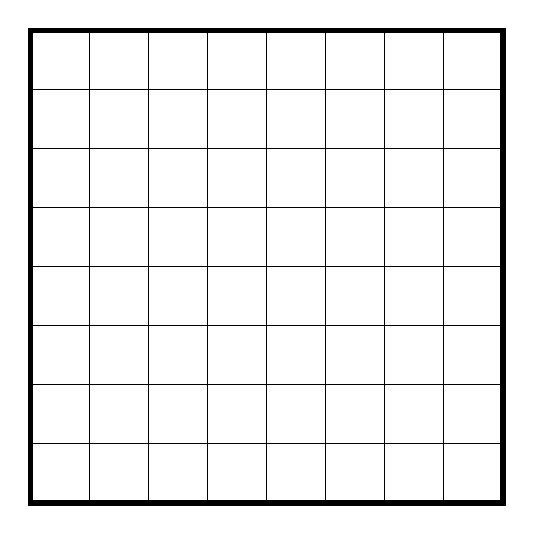
\begin{tikzpicture}[scale=0.75]

\foreach \a in {0,...,8}{
	\draw (\a,0)--(\a,8);
	\draw (0,\a)--(8,\a);
}

\draw[line width = 2] (0,0)--(8,0)--(8,8)--(0,8)--cycle;

\end{tikzpicture} \\ 
And I wonder why this particular shape is so essential: \\
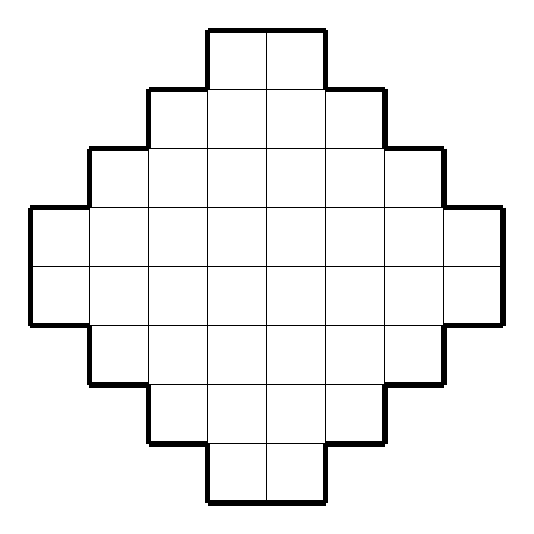
\begin{tikzpicture}[scale=0.75]



\foreach \a in {0,...,3}{

	\draw[line width=2] (\a  ,4-\a)--(\a+1, 4-\a  );
	\draw[line width=2] (\a+1,4-\a)--(\a+1, 4-\a-1);
	
	\draw (   \a, 4-\a)--(   \a, \a-4);
	\draw (-1*\a, 4-\a)--(-1*\a, \a-4);
	
	\draw ( 4-\a,    \a)--(\a-4,    \a);
	\draw ( 4-\a, -1*\a)--(\a-4, -1*\a);

	\def \b {-1}
	\def \c { 1}
		
	\draw[line width=2] (\b*\a  ,\c*4-\c*\a)--(\b*\a+\b*1, \c*4-\c*\a  );
	\draw[line width=2] (\b*\a+\b*1,\c*4-\c*\a)--(\b*\a+\b*1, \c*4-\c*\a-\c*1);
	
	\def \b { 1}
	\def \c {-1}
		
	\draw[line width=2] (\b*\a  ,\c*4-\c*\a)--(\b*\a+\b*1, \c*4-\c*\a  );
	\draw[line width=2] (\b*\a+\b*1,\c*4-\c*\a)--(\b*\a+\b*1, \c*4-\c*\a-\c*1);
	
	\def \b {-1}
	\def \c {-1}
		
	\draw[line width=2] (\b*\a  ,\c*4-\c*\a)--(\b*\a+\b*1, \c*4-\c*\a  );
	\draw[line width=2] (\b*\a+\b*1,\c*4-\c*\a)--(\b*\a+\b*1, \c*4-\c*\a-\c*1);

}

\end{tikzpicture}

\newpage

\noindent Pathetic Tutorial:

\fontfamily{qag}\selectfont \fontsize{12}{10}\selectfont

\begin{verbatim}
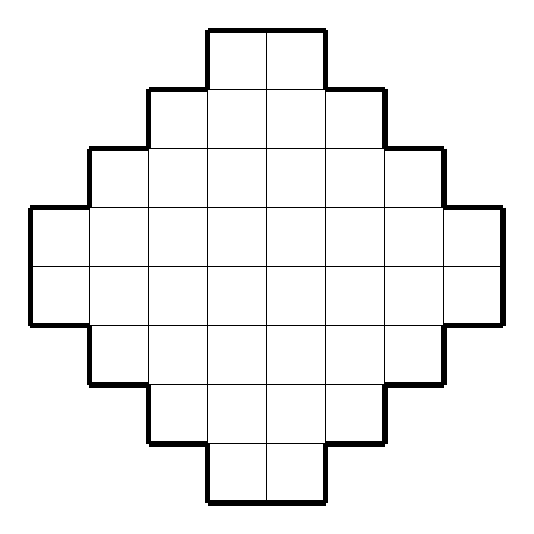
\begin{tikzpicture}[scale=0.75]

\foreach \a in {0,...,3}{

	\draw[line width=2] (\a  ,4-\a)--(\a+1, 4-\a  );
	\draw[line width=2] (\a+1,4-\a)--(\a+1, 4-\a-1);
	
	\draw (   \a, 4-\a)--(   \a, \a-4);
	\draw (-1*\a, 4-\a)--(-1*\a, \a-4);
	
	\draw ( 4-\a,    \a)--(\a-4,    \a);
	\draw ( 4-\a, -1*\a)--(\a-4, -1*\a);

	\def \b {-1}
	\def \c { 1}
		
	\draw[line width=2] (\b*\a     ,\c*4-\c*\a)--(\b*\a+\b*1, \c*4-\c*\a     );
	\draw[line width=2] (\b*\a+\b*1,\c*4-\c*\a)--(\b*\a+\b*1, \c*4-\c*\a-\c*1);
	
	\def \b { 1}
	\def \c {-1}
		
	\draw[line width=2] (\b*\a     ,\c*4-\c*\a)--(\b*\a+\b*1, \c*4-\c*\a     );
	\draw[line width=2] (\b*\a+\b*1,\c*4-\c*\a)--(\b*\a+\b*1, \c*4-\c*\a-\c*1);
	
	\def \b {-1}
	\def \c {-1}
		
	\draw[line width=2] (\b*\a     ,\c*4-\c*\a)--(\b*\a+\b*1, \c*4-\c*\a     );
	\draw[line width=2] (\b*\a+\b*1,\c*4-\c*\a)--(\b*\a+\b*1, \c*4-\c*\a-\c*1);

}

\end{tikzpicture}

\end{verbatim}


\noindent In French the word for tiling is \textit{pavage} -- so literally we are \textbf{paving} the shapes with dominoes. 




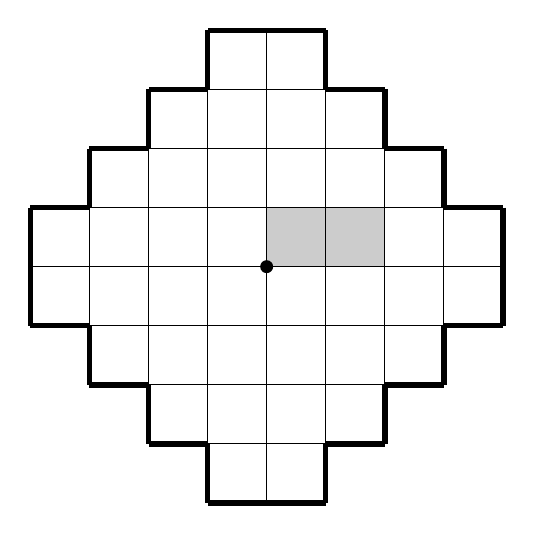
\begin{tikzpicture}[scale=0.75]

\def \b {0}
\def \c {0}


\draw[fill=black!20!white] (\b,\c)--(\b+2,\c)--(\b+2,\c+1)--(\b,\c+1)--cycle;
\draw[fill=black] (\b,\c) circle (0.1);

\foreach \a in {0,...,3}{

	\draw[line width=2] (\a  ,4-\a)--(\a+1, 4-\a  );
	\draw[line width=2] (\a+1,4-\a)--(\a+1, 4-\a-1);
	
	\draw (   \a, 4-\a)--(   \a, \a-4);
	\draw (-1*\a, 4-\a)--(-1*\a, \a-4);
	
	\draw ( 4-\a,    \a)--(\a-4,    \a);
	\draw ( 4-\a, -1*\a)--(\a-4, -1*\a);

	\def \b {-1}
	\def \c { 1}
		
	\draw[line width=2] (\b*\a  ,\c*4-\c*\a)--(\b*\a+\b*1, \c*4-\c*\a  );
	\draw[line width=2] (\b*\a+\b*1,\c*4-\c*\a)--(\b*\a+\b*1, \c*4-\c*\a-\c*1);
	
	\def \b { 1}
	\def \c {-1}
		
	\draw[line width=2] (\b*\a  ,\c*4-\c*\a)--(\b*\a+\b*1, \c*4-\c*\a  );
	\draw[line width=2] (\b*\a+\b*1,\c*4-\c*\a)--(\b*\a+\b*1, \c*4-\c*\a-\c*1);
	
	\def \b {-1}
	\def \c {-1}
		
	\draw[line width=2] (\b*\a  ,\c*4-\c*\a)--(\b*\a+\b*1, \c*4-\c*\a  );
	\draw[line width=2] (\b*\a+\b*1,\c*4-\c*\a)--(\b*\a+\b*1, \c*4-\c*\a-\c*1);

}

\end{tikzpicture}

\newpage

\noindent Let's put two reasonable tilings on the board.  One strategy for this shape is to start from the corners and work indwards.  And in this case we get lucky: it always works. \\

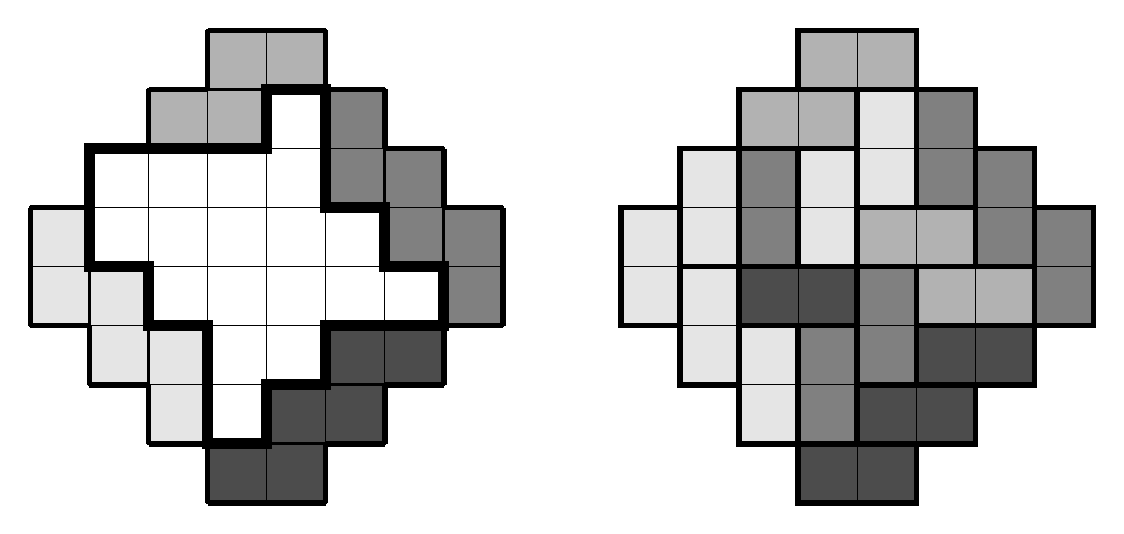
\begin{tikzpicture}[scale=0.75]


%\def \b {0}
%\def \c {0}
%\draw[fill=black!30!white, line width=2] (\b,\c)--(\b+2,\c)--(\b+2,\c+1)--(\b,\c+1)--cycle;

\def \b {-1}
\def \c {3}
\draw[fill=black!30!white, line width=1] (\b,\c)--(\b+2,\c)--(\b+2,\c+1)--(\b,\c+1)--cycle;

\def \b {-2}
\def \c {2}
\draw[fill=black!30!white, line width=1] (\b,\c)--(\b+2,\c)--(\b+2,\c+1)--(\b,\c+1)--cycle;

\def \b {-1}
\def \c {-4}
\draw[fill=black!70!white, line width=1] (\b,\c)--(\b+2,\c)--(\b+2,\c+1)--(\b,\c+1)--cycle;

\def \b {0}
\def \c {-3}
\draw[fill=black!70!white, line width=1] (\b,\c)--(\b+2,\c)--(\b+2,\c+1)--(\b,\c+1)--cycle;

\def \b {1}
\def \c {-2}
\draw[fill=black!70!white, line width=1] (\b,\c)--(\b+2,\c)--(\b+2,\c+1)--(\b,\c+1)--cycle;

\def \b {-4}
\def \c {-1}
\draw[fill=black!10!white, line width=1] (\b,\c)--(\b+1,\c)--(\b+1,\c+2)--(\b,\c+2)--cycle;

\def \b {-3}
\def \c {-2}
\draw[fill=black!10!white, line width=1] (\b,\c)--(\b+1,\c)--(\b+1,\c+2)--(\b,\c+2)--cycle;

\def \b {-2}
\def \c {-3}
\draw[fill=black!10!white, line width=1] (\b,\c)--(\b+1,\c)--(\b+1,\c+2)--(\b,\c+2)--cycle;

%\def \b {-3}
%\def \c {0}
%\draw[fill=black!10!white, line width=2] (\b,\c)--(\b+1,\c)--(\b+1,\c+2)--(\b,\c+2)--cycle;

\def \b {1}
\def \c {1}
\draw[fill=black!50!white, line width=1] (\b,\c)--(\b+1,\c)--(\b+1,\c+2)--(\b,\c+2)--cycle;

\def \b {2}
\def \c {0}
\draw[fill=black!50!white, line width=1] (\b,\c)--(\b+1,\c)--(\b+1,\c+2)--(\b,\c+2)--cycle;

\def \b {3}
\def \c {-1}
\draw[fill=black!50!white, line width=1] (\b,\c)--(\b+1,\c)--(\b+1,\c+2)--(\b,\c+2)--cycle;



\foreach \a in {0,...,3}{

	\draw[line width=2] (\a  ,4-\a)--(\a+1, 4-\a  );
	\draw[line width=2] (\a+1,4-\a)--(\a+1, 4-\a-1);
	
	\draw (   \a, 4-\a)--(   \a, \a-4);
	\draw (-1*\a, 4-\a)--(-1*\a, \a-4);
	
	\draw ( 4-\a,    \a)--(\a-4,    \a);
	\draw ( 4-\a, -1*\a)--(\a-4, -1*\a);

	\def \b {-1}
	\def \c { 1}
		
	\draw[line width=2] (\b*\a  ,\c*4-\c*\a)--(\b*\a+\b*1, \c*4-\c*\a  );
	\draw[line width=2] (\b*\a+\b*1,\c*4-\c*\a)--(\b*\a+\b*1, \c*4-\c*\a-\c*1);
	
	\def \b { 1}
	\def \c {-1}
		
	\draw[line width=2] (\b*\a  ,\c*4-\c*\a)--(\b*\a+\b*1, \c*4-\c*\a  );
	\draw[line width=2] (\b*\a+\b*1,\c*4-\c*\a)--(\b*\a+\b*1, \c*4-\c*\a-\c*1);
	
	\def \b {-1}
	\def \c {-1}
		
	\draw[line width=2] (\b*\a  ,\c*4-\c*\a)--(\b*\a+\b*1, \c*4-\c*\a  );
	\draw[line width=2] (\b*\a+\b*1,\c*4-\c*\a)--(\b*\a+\b*1, \c*4-\c*\a-\c*1);

}

\draw[line width=4] (0,-2)--(1,-2)--(1,-1)--(3,-1)--(3,0)--(2,0)--(2,1)--(1,1)--(1,3)--(0,3)--(0,2)--(-3,2)--(-3,0)--(-2,0)--(-2,-1)--(-1,-1)--(-1,-3)--(0,-3)--cycle;

\begin{scope}[xshift=10cm]

%\def \b {0}
%\def \c {0}
%\draw[fill=black!30!white, line width=2] (\b,\c)--(\b+2,\c)--(\b+2,\c+1)--(\b,\c+1)--cycle;

\def \b {-1}
\def \c {3}
\draw[fill=black!30!white, line width=2] (\b,\c)--(\b+2,\c)--(\b+2,\c+1)--(\b,\c+1)--cycle;

\def \b {-2}
\def \c {2}
\draw[fill=black!30!white, line width=2] (\b,\c)--(\b+2,\c)--(\b+2,\c+1)--(\b,\c+1)--cycle;

\def \b {1}
\def \c {-1}
\draw[fill=black!30!white, line width=2] (\b,\c)--(\b+2,\c)--(\b+2,\c+1)--(\b,\c+1)--cycle;

\def \b {0}
\def \c {0}
\draw[fill=black!30!white, line width=2] (\b,\c)--(\b+2,\c)--(\b+2,\c+1)--(\b,\c+1)--cycle;

\def \b {-1}
\def \c {-4}
\draw[fill=black!70!white, line width=2] (\b,\c)--(\b+2,\c)--(\b+2,\c+1)--(\b,\c+1)--cycle;

\def \b {0}
\def \c {-3}
\draw[fill=black!70!white, line width=2] (\b,\c)--(\b+2,\c)--(\b+2,\c+1)--(\b,\c+1)--cycle;

\def \b {1}
\def \c {-2}
\draw[fill=black!70!white, line width=2] (\b,\c)--(\b+2,\c)--(\b+2,\c+1)--(\b,\c+1)--cycle;

\def \b {-2}
\def \c {-1}
\draw[fill=black!70!white, line width=2] (\b,\c)--(\b+2,\c)--(\b+2,\c+1)--(\b,\c+1)--cycle;

\def \b {-4}
\def \c {-1}
\draw[fill=black!10!white, line width=2] (\b,\c)--(\b+1,\c)--(\b+1,\c+2)--(\b,\c+2)--cycle;

\def \b {-3}
\def \c {-2}
\draw[fill=black!10!white, line width=2] (\b,\c)--(\b+1,\c)--(\b+1,\c+2)--(\b,\c+2)--cycle;

\def \b {-2}
\def \c {-3}
\draw[fill=black!10!white, line width=2] (\b,\c)--(\b+1,\c)--(\b+1,\c+2)--(\b,\c+2)--cycle;

\def \b {0}
\def \c {1}
\draw[fill=black!10!white, line width=2] (\b,\c)--(\b+1,\c)--(\b+1,\c+2)--(\b,\c+2)--cycle;

\def \b {-3}
\def \c {0}
\draw[fill=black!10!white, line width=2] (\b,\c)--(\b+1,\c)--(\b+1,\c+2)--(\b,\c+2)--cycle;

\def \b {-1}
\def \c {0}
\draw[fill=black!10!white, line width=2] (\b,\c)--(\b+1,\c)--(\b+1,\c+2)--(\b,\c+2)--cycle;

\def \b {1}
\def \c {1}
\draw[fill=black!50!white, line width=2] (\b,\c)--(\b+1,\c)--(\b+1,\c+2)--(\b,\c+2)--cycle;

\def \b {2}
\def \c {0}
\draw[fill=black!50!white, line width=2] (\b,\c)--(\b+1,\c)--(\b+1,\c+2)--(\b,\c+2)--cycle;

\def \b {3}
\def \c {-1}
\draw[fill=black!50!white, line width=2] (\b,\c)--(\b+1,\c)--(\b+1,\c+2)--(\b,\c+2)--cycle;

\def \b {-2}
\def \c {0}
\draw[fill=black!50!white, line width=2] (\b,\c)--(\b+1,\c)--(\b+1,\c+2)--(\b,\c+2)--cycle;

\def \b {-1}
\def \c {-3}
\draw[fill=black!50!white, line width=2] (\b,\c)--(\b+1,\c)--(\b+1,\c+2)--(\b,\c+2)--cycle;

\def \b {0}
\def \c {-2}
\draw[fill=black!50!white, line width=2] (\b,\c)--(\b+1,\c)--(\b+1,\c+2)--(\b,\c+2)--cycle;

\foreach \a in {0,...,3}{

	\draw[line width=2] (\a  ,4-\a)--(\a+1, 4-\a  );
	\draw[line width=2] (\a+1,4-\a)--(\a+1, 4-\a-1);
	
	\draw (   \a, 4-\a)--(   \a, \a-4);
	\draw (-1*\a, 4-\a)--(-1*\a, \a-4);
	
	\draw ( 4-\a,    \a)--(\a-4,    \a);
	\draw ( 4-\a, -1*\a)--(\a-4, -1*\a);

	\def \b {-1}
	\def \c { 1}
		
	\draw[line width=2] (\b*\a  ,\c*4-\c*\a)--(\b*\a+\b*1, \c*4-\c*\a  );
	\draw[line width=2] (\b*\a+\b*1,\c*4-\c*\a)--(\b*\a+\b*1, \c*4-\c*\a-\c*1);
	
	\def \b { 1}
	\def \c {-1}
		
	\draw[line width=2] (\b*\a  ,\c*4-\c*\a)--(\b*\a+\b*1, \c*4-\c*\a  );
	\draw[line width=2] (\b*\a+\b*1,\c*4-\c*\a)--(\b*\a+\b*1, \c*4-\c*\a-\c*1);
	
	\def \b {-1}
	\def \c {-1}
		
	\draw[line width=2] (\b*\a  ,\c*4-\c*\a)--(\b*\a+\b*1, \c*4-\c*\a  );
	\draw[line width=2] (\b*\a+\b*1,\c*4-\c*\a)--(\b*\a+\b*1, \c*4-\c*\a-\c*1);

}

\end{scope}

\end{tikzpicture} \\ 

\noindent And for rectangle the case is even clearer.  There are no intermediate stages.  I mean, if you put enough tiles down there can be come question as to whether you put yourself in a corner yet.   \\ \\

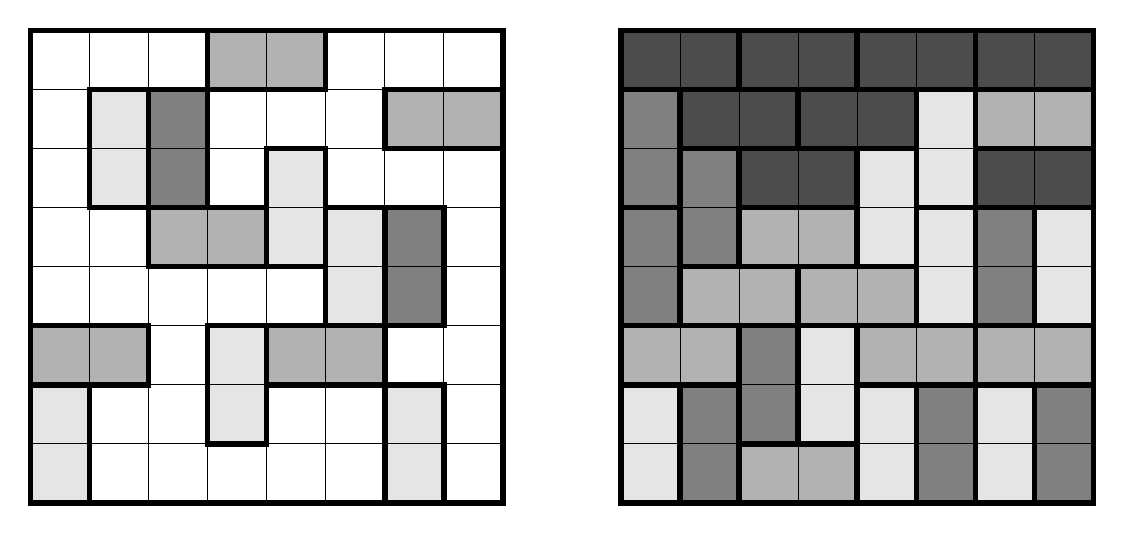
\begin{tikzpicture}[scale=0.75]

\def \b {0}
\def \c {0}
\draw[fill=black!10!white, line width=2] (\b,\c)--(\b+1,\c)--(\b+1,\c+2)--(\b,\c+2)--cycle;

\def \b {3}
\def \c {1}
\draw[fill=black!10!white, line width=2] (\b,\c)--(\b+1,\c)--(\b+1,\c+2)--(\b,\c+2)--cycle;

\def \b {4}
\def \c {4}
\draw[fill=black!10!white, line width=2] (\b,\c)--(\b+1,\c)--(\b+1,\c+2)--(\b,\c+2)--cycle;

\def \b {5}
\def \c {3}
\draw[fill=black!10!white, line width=2] (\b,\c)--(\b+1,\c)--(\b+1,\c+2)--(\b,\c+2)--cycle;

\def \b {6}
\def \c {0}
\draw[fill=black!10!white, line width=2] (\b,\c)--(\b+1,\c)--(\b+1,\c+2)--(\b,\c+2)--cycle;

\def \b {1}
\def \c {5}
\draw[fill=black!10!white, line width=2] (\b,\c)--(\b+1,\c)--(\b+1,\c+2)--(\b,\c+2)--cycle;

\def \b {0}
\def \c {2}
\draw[fill=black!30!white, line width=2] (\b,\c)--(\b+2,\c)--(\b+2,\c+1)--(\b,\c+1)--cycle;

\def \b {2}
\def \c {4}
\draw[fill=black!30!white, line width=2] (\b,\c)--(\b+2,\c)--(\b+2,\c+1)--(\b,\c+1)--cycle;

\def \b {3}
\def \c {7}
\draw[fill=black!30!white, line width=2] (\b,\c)--(\b+2,\c)--(\b+2,\c+1)--(\b,\c+1)--cycle;

\def \b {6}
\def \c {6}
\draw[fill=black!30!white, line width=2] (\b,\c)--(\b+2,\c)--(\b+2,\c+1)--(\b,\c+1)--cycle;

\def \b {4}
\def \c {2}
\draw[fill=black!30!white, line width=2] (\b,\c)--(\b+2,\c)--(\b+2,\c+1)--(\b,\c+1)--cycle;

\def \b {6}
\def \c {3}
\draw[fill=black!50!white, line width=2] (\b,\c)--(\b+1,\c)--(\b+1,\c+2)--(\b,\c+2)--cycle;

\def \b {2}
\def \c {5}
\draw[fill=black!50!white, line width=2] (\b,\c)--(\b+1,\c)--(\b+1,\c+2)--(\b,\c+2)--cycle;

\foreach \a in {0,...,8}{
	\draw (\a,0)--(\a,8);
	\draw (0,\a)--(8,\a);
}

\draw[line width = 2] (0,0)--(8,0)--(8,8)--(0,8)--cycle;



\begin{scope}[xshift=10cm]

\def \b {0}
\def \c {0}
\draw[fill=black!10!white, line width=2] (\b,\c)--(\b+1,\c)--(\b+1,\c+2)--(\b,\c+2)--cycle;

\def \b {3}
\def \c {1}
\draw[fill=black!10!white, line width=2] (\b,\c)--(\b+1,\c)--(\b+1,\c+2)--(\b,\c+2)--cycle;

\def \b {4}
\def \c {4}
\draw[fill=black!10!white, line width=2] (\b,\c)--(\b+1,\c)--(\b+1,\c+2)--(\b,\c+2)--cycle;

\def \b {5}
\def \c {3}
\draw[fill=black!10!white, line width=2] (\b,\c)--(\b+1,\c)--(\b+1,\c+2)--(\b,\c+2)--cycle;

\def \b {6}
\def \c {0}
\draw[fill=black!10!white, line width=2] (\b,\c)--(\b+1,\c)--(\b+1,\c+2)--(\b,\c+2)--cycle;

\def \b {1}
\def \c {5}
%\draw[fill=black!10!white, line width=2] (\b,\c)--(\b+1,\c)--(\b+1,\c+2)--(\b,\c+2)--cycle;

\def \b {0}
\def \c {2}
\draw[fill=black!30!white, line width=2] (\b,\c)--(\b+2,\c)--(\b+2,\c+1)--(\b,\c+1)--cycle;

\def \b {2}
\def \c {4}
\draw[fill=black!30!white, line width=2] (\b,\c)--(\b+2,\c)--(\b+2,\c+1)--(\b,\c+1)--cycle;

\def \b {2}
\def \c {7}
\draw[fill=black!70!white, line width=2] (\b,\c)--(\b+2,\c)--(\b+2,\c+1)--(\b,\c+1)--cycle;


\def \b {4}
\def \c {7}
\draw[fill=black!70!white, line width=2] (\b,\c)--(\b+2,\c)--(\b+2,\c+1)--(\b,\c+1)--cycle;

\def \b {3}
\def \c {6}
\draw[fill=black!70!white, line width=2] (\b,\c)--(\b+2,\c)--(\b+2,\c+1)--(\b,\c+1)--cycle;

\def \b {2}
\def \c {5}
\draw[fill=black!70!white, line width=2] (\b,\c)--(\b+2,\c)--(\b+2,\c+1)--(\b,\c+1)--cycle;

\def \b {1}
\def \c {6}
\draw[fill=black!70!white, line width=2] (\b,\c)--(\b+2,\c)--(\b+2,\c+1)--(\b,\c+1)--cycle;

\def \b {0}
\def \c {7}
\draw[fill=black!70!white, line width=2] (\b,\c)--(\b+2,\c)--(\b+2,\c+1)--(\b,\c+1)--cycle;


\def \b {6}
\def \c {6}
\draw[fill=black!30!white, line width=2] (\b,\c)--(\b+2,\c)--(\b+2,\c+1)--(\b,\c+1)--cycle;

\def \b {4}
\def \c {2}
\draw[fill=black!30!white, line width=2] (\b,\c)--(\b+2,\c)--(\b+2,\c+1)--(\b,\c+1)--cycle;

\def \b {6}
\def \c {3}
\draw[fill=black!50!white, line width=2] (\b,\c)--(\b+1,\c)--(\b+1,\c+2)--(\b,\c+2)--cycle;

\def \b {2}
\def \c {5}
%\draw[fill=black!50!white, line width=2] (\b,\c)--(\b+1,\c)--(\b+1,\c+2)--(\b,\c+2)--cycle;

\def \b {7}
\def \c {0}
\draw[fill=black!50!white, line width=2] (\b,\c)--(\b+1,\c)--(\b+1,\c+2)--(\b,\c+2)--cycle;

\def \b {6}
\def \c {2}
\draw[fill=black!30!white, line width=2] (\b,\c)--(\b+2,\c)--(\b+2,\c+1)--(\b,\c+1)--cycle;

\def \b {7}
\def \c {3}
\draw[fill=black!10!white, line width=2] (\b,\c)--(\b+1,\c)--(\b+1,\c+2)--(\b,\c+2)--cycle;

\def \b {6}
\def \c {5}
\draw[fill=black!70!white, line width=2] (\b,\c)--(\b+2,\c)--(\b+2,\c+1)--(\b,\c+1)--cycle;

\def \b {6}
\def \c {7}
\draw[fill=black!70!white, line width=2] (\b,\c)--(\b+2,\c)--(\b+2,\c+1)--(\b,\c+1)--cycle;

\def \b {5}
\def \c {5}
\draw[fill=black!10!white, line width=2] (\b,\c)--(\b+1,\c)--(\b+1,\c+2)--(\b,\c+2)--cycle;

\def \b {5}
\def \c {0}
\draw[fill=black!50!white, line width=2] (\b,\c)--(\b+1,\c)--(\b+1,\c+2)--(\b,\c+2)--cycle;

\def \b {4}
\def \c {0}
\draw[fill=black!10!white, line width=2] (\b,\c)--(\b+1,\c)--(\b+1,\c+2)--(\b,\c+2)--cycle;

\def \b {3}
\def \c {3}
\draw[fill=black!30!white, line width=2] (\b,\c)--(\b+2,\c)--(\b+2,\c+1)--(\b,\c+1)--cycle;

\def \b {2}
\def \c {0}
\draw[fill=black!30!white, line width=2] (\b,\c)--(\b+2,\c)--(\b+2,\c+1)--(\b,\c+1)--cycle;

\def \b {1}
\def \c {0}
\draw[fill=black!50!white, line width=2] (\b,\c)--(\b+1,\c)--(\b+1,\c+2)--(\b,\c+2)--cycle;

\def \b {2}
\def \c {1}
\draw[fill=black!50!white, line width=2] (\b,\c)--(\b+1,\c)--(\b+1,\c+2)--(\b,\c+2)--cycle;

\def \b {1}
\def \c {3}
\draw[fill=black!30!white, line width=2] (\b,\c)--(\b+2,\c)--(\b+2,\c+1)--(\b,\c+1)--cycle;

\def \b {0}
\def \c {3}
\draw[fill=black!50!white, line width=2] (\b,\c)--(\b+1,\c)--(\b+1,\c+2)--(\b,\c+2)--cycle;

\def \b {0}
\def \c {5}
\draw[fill=black!50!white, line width=2] (\b,\c)--(\b+1,\c)--(\b+1,\c+2)--(\b,\c+2)--cycle;

\def \b {1}
\def \c {4}
\draw[fill=black!50!white, line width=2] (\b,\c)--(\b+1,\c)--(\b+1,\c+2)--(\b,\c+2)--cycle;

\foreach \a in {0,...,8}{
	\draw (\a,0)--(\a,8);
	\draw (0,\a)--(8,\a);
}

\draw[line width = 2] (0,0)--(8,0)--(8,8)--(0,8)--cycle;

\end{scope}


\end{tikzpicture} \\ \\
There is also the lovely John Conway game of ``Domineering" which is not related but you also place dominoes on a checkerboard. See \textbf{Winning Ways for Your Mathematical Plays} (Vol I). \\ \\
\textbf{Exercise} Fill the rest of the tiling. \\ \\
\textbf{Answer} There is no solution, but if you move the tiles slightly (actually quite a bit here...) you can get a problem with an answer.  \\ \\
The number of tilings on the top looks atypical -- just purely on a hunch.  Where did that hunch come from? Is it right? \\ \\
As with all hunches, it can be proven with hundreds of pages of equations this tiling is not likely to appear in a rectangles.  We'll settle for somewhat simpler patterns. 

\newpage

\noindent 

\newpage 

\noindent Next I hav to address some redundancy.  Every couple of years, it seems there were more and more people who came up with a similar theory and did not talk to each other.



\begin{itemize}
\item \textbf{domino tilings} 
\item dimer model 
\item perfect matchings
\item \textbf{six-vertex  model}
\item Alternating Sign Matrix (\textbf{ASM})
\item XXZ spin chain
\item Ising model
\end{itemize}

\noindent Domino tilings and six-vertex are closely related.  You can see the family resemblance.  

\includegraphics[width=5in]{AD-05.png} \\

\noindent For every 6-vertex configuration there is a domino tiling, up to various factors of $\times 2$.  

\includegraphics[width=5in]{AD-06.png}\\
The Aztec Diamond is a natural shape because it \textbf{is} the square lattice.

\newpage

\fontfamily{qag}\selectfont \fontsize{20}{25}\selectfont  

\noindent \textbf{Problem Session} Let us compute some square-ice and domino tiling partition functions! 


\vfill

\fontfamily{qag}\selectfont \fontsize{12}{10}\selectfont

\begin{thebibliography}{}

\item Paul Zinn-Justin \textbf{Six-Vertex Model with Domain Wall Boundary Conditions and One-Matrix Model} \texttt{arXiv:math-ph/0005008}

\item Noam Elkies, Greg Kuperberg, Michael Larsen, James Propp \\ \textbf{Alternating-Sign Matrices and Domino Tilings (Part I) }  \\ Journal of Algebraic Combinatorics (1992) 1: 111.  \texttt{doi:10.1023/A:1022420103267}

\item Patrick Ferrari, Herbert Spohn \textbf{Domino tilings and the six-vertex model at its free fermion point} \texttt{arXiv:cond-mat/0605406}

\item Sunil Chhita, Kurt Johansson \textbf{Domino statistics of the two-periodic Aztec diamond} \texttt{arXiv:1410.2385
}

\end{thebibliography} 




\newpage

\fontfamily{qag}\selectfont \fontsize{20}{25}\selectfont  

\noindent \textbf{Big Idea} \\ \\
The link between the domino tilings and the ising model is ``well known" but I can never find out all the details I want.  And if I ask the question, it doesn't have any merit. \\ \\
Who are we to believe?  \\ \\
There are actually \textit{two} Ising models.  The statistical Ising model and the Ising Conformal Field Theories. \\ \\ 
The bad news is, statistical models -- or maybe, \textbf{lattice gauge theories}.  Here's a simple question: {\color{blue!50!green}are domino tilings an instance of lattice gauge theory}? The answer is likely ``yes" but all of the responses are wanting. \\ \\
The domino tilings like I have been showing you?  Which lattice gauge theory was that?  Domino tilings is very simple, lattice gauge theory rather involved.  

\includegraphics[width=5in]{AD-07.png} \\
The Ising model is even more simple-minded than the domino tilings.  How could it be so advanced? 

\newpage

\noindent One way to count the domino tilings is through the Kasteleyn determinant.  In the $2 \times 2$ square, there are 4 vertices: \\
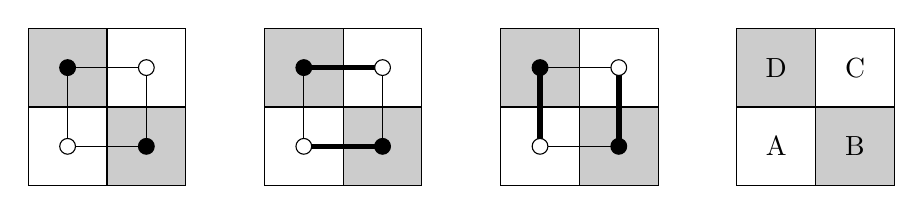
\begin{tikzpicture}

\def \domino {

	\def \a {0}
	\def \b {0}
	\draw (\a,\b)--(\a+1,\b)--(\a+1,\b+1)--(\a,\b+1)--cycle;

	\def \a {1}
	\def \b {0}
	\draw[fill=black!20!white] (\a,\b)--(\a+1,\b)--(\a+1,\b+1)--(\a,\b+1)--cycle;

	\def \a {0}
	\def \b {1}
	\draw[fill=black!20!white] (\a,\b)--(\a+1,\b)--(\a+1,\b+1)--(\a,\b+1)--cycle;

	\def \a {1}
	\def \b {1}
	\draw (\a,\b)--(\a+1,\b)--(\a+1,\b+1)--(\a,\b+1)--cycle;

}

% ------------------------------------------------------

\def \dimer {

	\draw (0.5,0.5)--(1.5,0.5)--(1.5,1.5)--(0.5,1.5)--cycle;

	\def \a {0}
	\def \b {0}
	\draw[fill=white] (\a + 0.5 ,\b + 0.5) circle (0.1);

	\def \a {1}
	\def \b {0}
	\draw[fill=black] (\a + 0.5 ,\b + 0.5) circle (0.1);

	\def \a {0}
	\def \b {1}
	\draw[fill=black] (\a + 0.5 ,\b + 0.5) circle (0.1);

	\def \a {1}
	\def \b {1}
	\draw[fill=white] (\a + 0.5 ,\b + 0.5) circle (0.1);

}

\domino

\dimer

\begin{scope}[xshift=3cm]

\domino

\draw[line width=2] (0.5,0.5)--(1.5,0.5);

\draw[line width=2] (0.5,1.5)--(1.5,1.5);

\dimer



\end{scope}

\begin{scope}[xshift=6cm]

\domino

\draw[line width=2] (0.5,0.5)--(0.5,1.5);

\draw[line width=2] (1.5,0.5)--(1.5,1.5);

\dimer

\end{scope}

\begin{scope}[xshift=9cm]

\domino

\node at (0.5,0.5) {A};

\node at (1.5,0.5) {B};

\node at (1.5,1.5) {C};

\node at (0.5,1.5) {D};

\end{scope}

\end{tikzpicture} \\ 
There should be two tilings.  Let's make sure Kateleyn's method returns the answer \textbf{2}.  He would draw a matrix:
$$ Pf \left[ \begin{array}{c|cccc}
 & \text{A} & \text{B} & \text{C} & \text{D} \\ \hline
\text{A} & 0 & 1 &  0 &  1 \\
\text{B} & 1 & 0 &  1 &  0 \\ 
\text{C} & 0 & 1 &  0 &  1 \\
\text{D} & 1 & 0 &  1 &  0 
 \end{array}\right] \stackrel{?}{=} Det 
 \left[ \begin{array}{c|cc}
 & \text{C} & \text{D} \\ \hline
\text{A} & 1 & 1  \\
\text{B} & 1 & 1  \\ 
 \end{array}\right]
 $$
Since A is next to B, the entry A-B is 1.  B and D are not next to each other.  And then we compute not the Determinant, but the Pfaffian. \\ \\
Hopefully the value of the Pfaffian is $2$.  The value of that determinant is $0$.
I guess I have to put a minus sign.

$$ \hspace{0.8in} Pf \left[ \begin{array}{c|cccc}
 & \text{A} & \text{B} & \text{C} & \text{D} \\ \hline
\text{A} & 0 & 1 &  0 &  1 \\
\text{B} & 1 & 0 &  1 &  0 \\ 
\text{C} & 0 & 1 &  0 &  1 \\
\text{D} & 1 & 0 &  1 &  0 
 \end{array}\right] = Det 
 \left[ \begin{array}{c|cr}
 & \text{C} & \text{D} \\ \hline
\text{A} & 1 & -1  \\
\text{B} & 1 & 1  \\ 
 \end{array}\right] = 2
 $$
We are just making it up as we go along and this is the Kasteleyn orientation. \\ \\ Without knowing why, this is just what we have to do in order to make sense, and this is called an ``anomaly".


\newpage

\noindent There should be ways to ``glue" the patches together and the number of domino tilings will behave in an organized way.  \\ \\
As for all this Ising model stuff.  As long as we know the ising model and the domino tilings are the same theory.  \\ \\The ising model has varied literature\footnote{The dilemma these are 4 very complicated topics, none of which I know very well, and we are trying to make a comparison.  Namely, the ising model literature is all over the place, there should be variants of the domino tilings as well, where the answers still make a lot of sense.} - all over the place:
\begin{itemize}
\item statistical mechanics
\item integrable systems
\item TQFT
\item lattice gauge theory
\item Chern Simons Theory
\end{itemize}
and yet we only except one tractable model, the domino tilings. We need more examples: \\
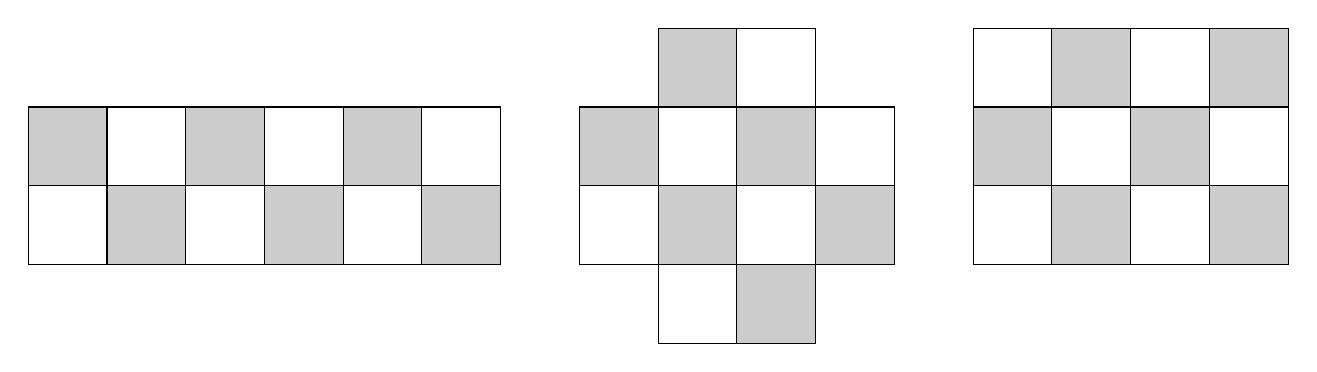
\begin{tikzpicture}

	\def \a {0}
	\def \b {0}
	\draw[fill=black!0!white] (\a,\b)--(\a+1,\b)--(\a+1,\b+1)--(\a,\b+1)--cycle;
	\def \a {1}
	\def \b {0}
	\draw[fill=black!20!white] (\a,\b)--(\a+1,\b)--(\a+1,\b+1)--(\a,\b+1)--cycle;
	\def \a {2}
	\def \b {0}
	\draw[fill=black!0!white] (\a,\b)--(\a+1,\b)--(\a+1,\b+1)--(\a,\b+1)--cycle;
	\def \a {3}
	\def \b {0}
	\draw[fill=black!20!white] (\a,\b)--(\a+1,\b)--(\a+1,\b+1)--(\a,\b+1)--cycle;
	\def \a {4}
	\def \b {0}
	\draw[fill=black!0!white] (\a,\b)--(\a+1,\b)--(\a+1,\b+1)--(\a,\b+1)--cycle;
	\def \a {5}
	\def \b {0}
	\draw[fill=black!20!white] (\a,\b)--(\a+1,\b)--(\a+1,\b+1)--(\a,\b+1)--cycle;
	\def \a {0}
	\def \b {1}
	\draw[fill=black!20!white] (\a,\b)--(\a+1,\b)--(\a+1,\b+1)--(\a,\b+1)--cycle;
	\def \a {1}
	\def \b {1}
	\draw[fill=black!0!white] (\a,\b)--(\a+1,\b)--(\a+1,\b+1)--(\a,\b+1)--cycle;
	\def \a {2}
	\def \b {1}
	\draw[fill=black!20!white] (\a,\b)--(\a+1,\b)--(\a+1,\b+1)--(\a,\b+1)--cycle;
	\def \a {3}
	\def \b {1}
	\draw[fill=black!0!white] (\a,\b)--(\a+1,\b)--(\a+1,\b+1)--(\a,\b+1)--cycle;
	\def \a {4}
	\def \b {1}
	\draw[fill=black!20!white] (\a,\b)--(\a+1,\b)--(\a+1,\b+1)--(\a,\b+1)--cycle;
	\def \a {5}
	\def \b {1}
	\draw[fill=black!0!white] (\a,\b)--(\a+1,\b)--(\a+1,\b+1)--(\a,\b+1)--cycle;
	
	
\begin{scope}[xshift=7cm]

	\def \a {0}
	\def \b {0}
	\draw[fill=black!0!white] (\a,\b)--(\a+1,\b)--(\a+1,\b+1)--(\a,\b+1)--cycle;
	\def \a {1}
	\def \b {0}
	\draw[fill=black!20!white] (\a,\b)--(\a+1,\b)--(\a+1,\b+1)--(\a,\b+1)--cycle;
	\def \a {2}
	\def \b {0}
	\draw[fill=black!0!white] (\a,\b)--(\a+1,\b)--(\a+1,\b+1)--(\a,\b+1)--cycle;
	\def \a {3}
	\def \b {0}
	\draw[fill=black!20!white] (\a,\b)--(\a+1,\b)--(\a+1,\b+1)--(\a,\b+1)--cycle;
	\def \a {0}
	\def \b {1}
	\draw[fill=black!20!white] (\a,\b)--(\a+1,\b)--(\a+1,\b+1)--(\a,\b+1)--cycle;
	\def \a {1}
	\def \b {1}
	\draw[fill=black!0!white] (\a,\b)--(\a+1,\b)--(\a+1,\b+1)--(\a,\b+1)--cycle;
	\def \a {2}
	\def \b {1}
	\draw[fill=black!20!white] (\a,\b)--(\a+1,\b)--(\a+1,\b+1)--(\a,\b+1)--cycle;
	\def \a {3}
	\def \b {1}
	\draw[fill=black!0!white] (\a,\b)--(\a+1,\b)--(\a+1,\b+1)--(\a,\b+1)--cycle;
	\def \a {1}
	\def \b {2}
	\draw[fill=black!20!white] (\a,\b)--(\a+1,\b)--(\a+1,\b+1)--(\a,\b+1)--cycle;
	\def \a {2}
	\def \b {2}
	\draw[fill=black!0!white] (\a,\b)--(\a+1,\b)--(\a+1,\b+1)--(\a,\b+1)--cycle;
	\def \a { 1}
	\def \b {-1}
	\draw[fill=black!0!white] (\a,\b)--(\a+1,\b)--(\a+1,\b+1)--(\a,\b+1)--cycle;
	\def \a { 2}
	\def \b {-1}
	\draw[fill=black!20!white] (\a,\b)--(\a+1,\b)--(\a+1,\b+1)--(\a,\b+1)--cycle;

\end{scope}

\begin{scope}[xshift=12cm]

	\def \a {0}
	\def \b {0}
	\draw[fill=black!0!white] (\a,\b)--(\a+1,\b)--(\a+1,\b+1)--(\a,\b+1)--cycle;
	\def \a {1}
	\def \b {0}
	\draw[fill=black!20!white] (\a,\b)--(\a+1,\b)--(\a+1,\b+1)--(\a,\b+1)--cycle;
	\def \a {2}
	\def \b {0}
	\draw[fill=black!0!white] (\a,\b)--(\a+1,\b)--(\a+1,\b+1)--(\a,\b+1)--cycle;
	\def \a {3}
	\def \b {0}
	\draw[fill=black!20!white] (\a,\b)--(\a+1,\b)--(\a+1,\b+1)--(\a,\b+1)--cycle;
	\def \a {0}
	\def \b {1}
	\draw[fill=black!20!white] (\a,\b)--(\a+1,\b)--(\a+1,\b+1)--(\a,\b+1)--cycle;
	\def \a {1}
	\def \b {1}
	\draw[fill=black!0!white] (\a,\b)--(\a+1,\b)--(\a+1,\b+1)--(\a,\b+1)--cycle;
	\def \a {2}
	\def \b {1}
	\draw[fill=black!20!white] (\a,\b)--(\a+1,\b)--(\a+1,\b+1)--(\a,\b+1)--cycle;
	\def \a {3}
	\def \b {1}
	\draw[fill=black!0!white] (\a,\b)--(\a+1,\b)--(\a+1,\b+1)--(\a,\b+1)--cycle;
	\def \a {0}
	\def \b {2}
	\draw[fill=black!0!white] (\a,\b)--(\a+1,\b)--(\a+1,\b+1)--(\a,\b+1)--cycle;
	\def \a {1}
	\def \b {2}
	\draw[fill=black!20!white] (\a,\b)--(\a+1,\b)--(\a+1,\b+1)--(\a,\b+1)--cycle;
	\def \a {2}
	\def \b {2}
	\draw[fill=black!0!white] (\a,\b)--(\a+1,\b)--(\a+1,\b+1)--(\a,\b+1)--cycle;
	\def \a {3}
	\def \b {2}
	\draw[fill=black!20!white] (\a,\b)--(\a+1,\b)--(\a+1,\b+1)--(\a,\b+1)--cycle;

\end{scope}

\end{tikzpicture} \\
Can we glue partial answers together into a big picture?  You can.  In a very complicated way.

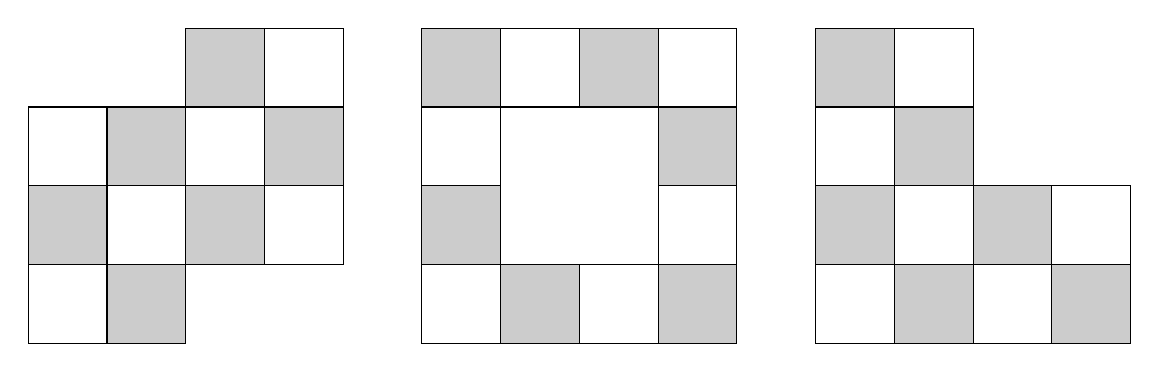
\begin{tikzpicture}


	\def \a {0}
	\def \b {0}
	\draw[fill=black!0!white] (\a,\b)--(\a+1,\b)--(\a+1,\b+1)--(\a,\b+1)--cycle;
	\def \a {1}
	\def \b {0}
	\draw[fill=black!20!white] (\a,\b)--(\a+1,\b)--(\a+1,\b+1)--(\a,\b+1)--cycle;
	\def \a {2}
	\def \b {1}
	\draw[fill=black!20!white] (\a,\b)--(\a+1,\b)--(\a+1,\b+1)--(\a,\b+1)--cycle;
	\def \a {3}
	\def \b {1}
	\draw[fill=black!0!white] (\a,\b)--(\a+1,\b)--(\a+1,\b+1)--(\a,\b+1)--cycle;
	\def \a {0}
	\def \b {1}
	\draw[fill=black!20!white] (\a,\b)--(\a+1,\b)--(\a+1,\b+1)--(\a,\b+1)--cycle;
	\def \a {1}
	\def \b {1}
	\draw[fill=black!0!white] (\a,\b)--(\a+1,\b)--(\a+1,\b+1)--(\a,\b+1)--cycle;
	\def \a {2}
	\def \b {2}
	\draw[fill=black!0!white] (\a,\b)--(\a+1,\b)--(\a+1,\b+1)--(\a,\b+1)--cycle;
	\def \a {3}
	\def \b {2}
	\draw[fill=black!20!white] (\a,\b)--(\a+1,\b)--(\a+1,\b+1)--(\a,\b+1)--cycle;
	\def \a {0}
	\def \b {2}
	\draw[fill=black!0!white] (\a,\b)--(\a+1,\b)--(\a+1,\b+1)--(\a,\b+1)--cycle;
	\def \a {1}
	\def \b {2}
	\draw[fill=black!20!white] (\a,\b)--(\a+1,\b)--(\a+1,\b+1)--(\a,\b+1)--cycle;
	\def \a {2}
	\def \b {3}
	\draw[fill=black!20!white] (\a,\b)--(\a+1,\b)--(\a+1,\b+1)--(\a,\b+1)--cycle;
	\def \a {3}
	\def \b {3}
	\draw[fill=black!0!white] (\a,\b)--(\a+1,\b)--(\a+1,\b+1)--(\a,\b+1)--cycle;


\begin{scope}[xshift=5cm]

	\def \a {0}
	\def \b {0}
	\draw[fill=black!0!white] (\a,\b)--(\a+1,\b)--(\a+1,\b+1)--(\a,\b+1)--cycle;
	\def \a {1}
	\def \b {0}
	\draw[fill=black!20!white] (\a,\b)--(\a+1,\b)--(\a+1,\b+1)--(\a,\b+1)--cycle;
	\def \a {2}
	\def \b {0}
	\draw[fill=black!0!white] (\a,\b)--(\a+1,\b)--(\a+1,\b+1)--(\a,\b+1)--cycle;
	\def \a {3}
	\def \b {0}
	\draw[fill=black!20!white] (\a,\b)--(\a+1,\b)--(\a+1,\b+1)--(\a,\b+1)--cycle;
	\def \a {3}
	\def \b {1}
	\draw[fill=black!0!white] (\a,\b)--(\a+1,\b)--(\a+1,\b+1)--(\a,\b+1)--cycle;
	\def \a {3}
	\def \b {2}
	\draw[fill=black!20!white] (\a,\b)--(\a+1,\b)--(\a+1,\b+1)--(\a,\b+1)--cycle;
	\def \a {3}
	\def \b {3}
	\draw[fill=black!0!white] (\a,\b)--(\a+1,\b)--(\a+1,\b+1)--(\a,\b+1)--cycle;
	\def \a {2}
	\def \b {3}
	\draw[fill=black!20!white] (\a,\b)--(\a+1,\b)--(\a+1,\b+1)--(\a,\b+1)--cycle;
	\def \a {1}
	\def \b {3}
	\draw[fill=black!0!white] (\a,\b)--(\a+1,\b)--(\a+1,\b+1)--(\a,\b+1)--cycle;
	\def \a {0}
	\def \b {3}
	\draw[fill=black!20!white] (\a,\b)--(\a+1,\b)--(\a+1,\b+1)--(\a,\b+1)--cycle;
	\def \a {0}
	\def \b {2}
	\draw[fill=black!0!white] (\a,\b)--(\a+1,\b)--(\a+1,\b+1)--(\a,\b+1)--cycle;
	\def \a {0}
	\def \b {1}
	\draw[fill=black!20!white] (\a,\b)--(\a+1,\b)--(\a+1,\b+1)--(\a,\b+1)--cycle;

\end{scope}

\begin{scope}[xshift=10cm]

	\def \a {0}
	\def \b {0}
	\draw[fill=black!0!white] (\a,\b)--(\a+1,\b)--(\a+1,\b+1)--(\a,\b+1)--cycle;
	\def \a {1}
	\def \b {0}
	\draw[fill=black!20!white] (\a,\b)--(\a+1,\b)--(\a+1,\b+1)--(\a,\b+1)--cycle;
	\def \a {2}
	\def \b {0}
	\draw[fill=black!0!white] (\a,\b)--(\a+1,\b)--(\a+1,\b+1)--(\a,\b+1)--cycle;
	\def \a {3}
	\def \b {0}
	\draw[fill=black!20!white] (\a,\b)--(\a+1,\b)--(\a+1,\b+1)--(\a,\b+1)--cycle;
	\def \a {0}
	\def \b {1}
	\draw[fill=black!20!white] (\a,\b)--(\a+1,\b)--(\a+1,\b+1)--(\a,\b+1)--cycle;
	\def \a {1}
	\def \b {1}
	\draw[fill=black!0!white] (\a,\b)--(\a+1,\b)--(\a+1,\b+1)--(\a,\b+1)--cycle;
	\def \a {2}
	\def \b {1}
	\draw[fill=black!20!white] (\a,\b)--(\a+1,\b)--(\a+1,\b+1)--(\a,\b+1)--cycle;
	\def \a {3}
	\def \b {1}
	\draw[fill=black!0!white] (\a,\b)--(\a+1,\b)--(\a+1,\b+1)--(\a,\b+1)--cycle;
	\def \a {0}
	\def \b {2}
	\draw[fill=black!0!white] (\a,\b)--(\a+1,\b)--(\a+1,\b+1)--(\a,\b+1)--cycle;
	\def \a {1}
	\def \b {2}
	\draw[fill=black!20!white] (\a,\b)--(\a+1,\b)--(\a+1,\b+1)--(\a,\b+1)--cycle;
	\def \a {0}
	\def \b {3}
	\draw[fill=black!20!white] (\a,\b)--(\a+1,\b)--(\a+1,\b+1)--(\a,\b+1)--cycle;
	\def \a {1}
	\def \b {3}
	\draw[fill=black!0!white] (\a,\b)--(\a+1,\b)--(\a+1,\b+1)--(\a,\b+1)--cycle;

\end{scope}

\end{tikzpicture} \\

\fontfamily{qag}\selectfont \fontsize{12}{10}\selectfont

\noindent An aside for the grown-ups.  The Kasteleyn determinants are put into a computer and with some effort the correct number will be returned.   In a sense, we have already used a tiny bit of cohomology theory.
\begin{itemize}
\item All of these shapes are homeomorphic (``the same as") $\mathbb{D}$ (all the rectangles are homomeomorphic.  The L-shapes are homeomorphic to rectangles).  This is a really myopic way of doing things and obviously loses important information.  
\item Fiddling with these shapes is essential.  The ``new" exercise here is to use the patchwork technique to check how the overlapping works.  
\end{itemize}

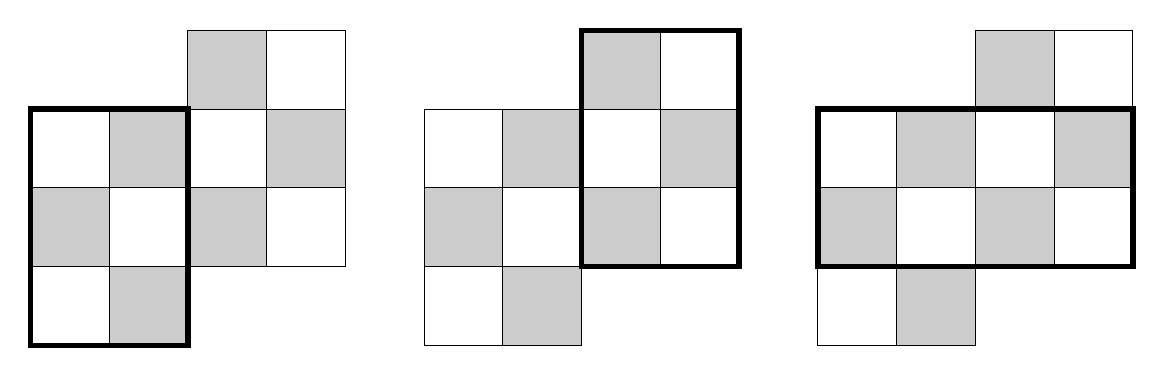
\begin{tikzpicture}

	\def \a {0}
	\def \b {0}
	\draw[fill=black!0!white] (\a,\b)--(\a+1,\b)--(\a+1,\b+1)--(\a,\b+1)--cycle;
	\def \a {1}
	\def \b {0}
	\draw[fill=black!20!white] (\a,\b)--(\a+1,\b)--(\a+1,\b+1)--(\a,\b+1)--cycle;
	\def \a {2}
	\def \b {1}
	\draw[fill=black!20!white] (\a,\b)--(\a+1,\b)--(\a+1,\b+1)--(\a,\b+1)--cycle;
	\def \a {3}
	\def \b {1}
	\draw[fill=black!0!white] (\a,\b)--(\a+1,\b)--(\a+1,\b+1)--(\a,\b+1)--cycle;
	\def \a {0}
	\def \b {1}
	\draw[fill=black!20!white] (\a,\b)--(\a+1,\b)--(\a+1,\b+1)--(\a,\b+1)--cycle;
	\def \a {1}
	\def \b {1}
	\draw[fill=black!0!white] (\a,\b)--(\a+1,\b)--(\a+1,\b+1)--(\a,\b+1)--cycle;
	\def \a {2}
	\def \b {2}
	\draw[fill=black!0!white] (\a,\b)--(\a+1,\b)--(\a+1,\b+1)--(\a,\b+1)--cycle;
	\def \a {3}
	\def \b {2}
	\draw[fill=black!20!white] (\a,\b)--(\a+1,\b)--(\a+1,\b+1)--(\a,\b+1)--cycle;
	\def \a {0}
	\def \b {2}
	\draw[fill=black!0!white] (\a,\b)--(\a+1,\b)--(\a+1,\b+1)--(\a,\b+1)--cycle;
	\def \a {1}
	\def \b {2}
	\draw[fill=black!20!white] (\a,\b)--(\a+1,\b)--(\a+1,\b+1)--(\a,\b+1)--cycle;
	\def \a {2}
	\def \b {3}
	\draw[fill=black!20!white] (\a,\b)--(\a+1,\b)--(\a+1,\b+1)--(\a,\b+1)--cycle;
	\def \a {3}
	\def \b {3}
	\draw[fill=black!0!white] (\a,\b)--(\a+1,\b)--(\a+1,\b+1)--(\a,\b+1)--cycle;
	
	\draw[line width=2] (0,0)--(2,0)--(2,3)--(0,3)--cycle;
	
\begin{scope}[xshift=5cm]

	\def \a {0}
	\def \b {0}
	\draw[fill=black!0!white] (\a,\b)--(\a+1,\b)--(\a+1,\b+1)--(\a,\b+1)--cycle;
	\def \a {1}
	\def \b {0}
	\draw[fill=black!20!white] (\a,\b)--(\a+1,\b)--(\a+1,\b+1)--(\a,\b+1)--cycle;
	\def \a {2}
	\def \b {1}
	\draw[fill=black!20!white] (\a,\b)--(\a+1,\b)--(\a+1,\b+1)--(\a,\b+1)--cycle;
	\def \a {3}
	\def \b {1}
	\draw[fill=black!0!white] (\a,\b)--(\a+1,\b)--(\a+1,\b+1)--(\a,\b+1)--cycle;
	\def \a {0}
	\def \b {1}
	\draw[fill=black!20!white] (\a,\b)--(\a+1,\b)--(\a+1,\b+1)--(\a,\b+1)--cycle;
	\def \a {1}
	\def \b {1}
	\draw[fill=black!0!white] (\a,\b)--(\a+1,\b)--(\a+1,\b+1)--(\a,\b+1)--cycle;
	\def \a {2}
	\def \b {2}
	\draw[fill=black!0!white] (\a,\b)--(\a+1,\b)--(\a+1,\b+1)--(\a,\b+1)--cycle;
	\def \a {3}
	\def \b {2}
	\draw[fill=black!20!white] (\a,\b)--(\a+1,\b)--(\a+1,\b+1)--(\a,\b+1)--cycle;
	\def \a {0}
	\def \b {2}
	\draw[fill=black!0!white] (\a,\b)--(\a+1,\b)--(\a+1,\b+1)--(\a,\b+1)--cycle;
	\def \a {1}
	\def \b {2}
	\draw[fill=black!20!white] (\a,\b)--(\a+1,\b)--(\a+1,\b+1)--(\a,\b+1)--cycle;
	\def \a {2}
	\def \b {3}
	\draw[fill=black!20!white] (\a,\b)--(\a+1,\b)--(\a+1,\b+1)--(\a,\b+1)--cycle;
	\def \a {3}
	\def \b {3}
	\draw[fill=black!0!white] (\a,\b)--(\a+1,\b)--(\a+1,\b+1)--(\a,\b+1)--cycle;
	
	\draw[line width=2] (2,1)--(4,1)--(4,4)--(2,4)--cycle;

\end{scope}

\begin{scope}[xshift=10cm]

	\def \a {0}
	\def \b {0}
	\draw[fill=black!0!white] (\a,\b)--(\a+1,\b)--(\a+1,\b+1)--(\a,\b+1)--cycle;
	\def \a {1}
	\def \b {0}
	\draw[fill=black!20!white] (\a,\b)--(\a+1,\b)--(\a+1,\b+1)--(\a,\b+1)--cycle;
	\def \a {2}
	\def \b {1}
	\draw[fill=black!20!white] (\a,\b)--(\a+1,\b)--(\a+1,\b+1)--(\a,\b+1)--cycle;
	\def \a {3}
	\def \b {1}
	\draw[fill=black!0!white] (\a,\b)--(\a+1,\b)--(\a+1,\b+1)--(\a,\b+1)--cycle;
	\def \a {0}
	\def \b {1}
	\draw[fill=black!20!white] (\a,\b)--(\a+1,\b)--(\a+1,\b+1)--(\a,\b+1)--cycle;
	\def \a {1}
	\def \b {1}
	\draw[fill=black!0!white] (\a,\b)--(\a+1,\b)--(\a+1,\b+1)--(\a,\b+1)--cycle;
	\def \a {2}
	\def \b {2}
	\draw[fill=black!0!white] (\a,\b)--(\a+1,\b)--(\a+1,\b+1)--(\a,\b+1)--cycle;
	\def \a {3}
	\def \b {2}
	\draw[fill=black!20!white] (\a,\b)--(\a+1,\b)--(\a+1,\b+1)--(\a,\b+1)--cycle;
	\def \a {0}
	\def \b {2}
	\draw[fill=black!0!white] (\a,\b)--(\a+1,\b)--(\a+1,\b+1)--(\a,\b+1)--cycle;
	\def \a {1}
	\def \b {2}
	\draw[fill=black!20!white] (\a,\b)--(\a+1,\b)--(\a+1,\b+1)--(\a,\b+1)--cycle;
	\def \a {2}
	\def \b {3}
	\draw[fill=black!20!white] (\a,\b)--(\a+1,\b)--(\a+1,\b+1)--(\a,\b+1)--cycle;
	\def \a {3}
	\def \b {3}
	\draw[fill=black!0!white] (\a,\b)--(\a+1,\b)--(\a+1,\b+1)--(\a,\b+1)--cycle;
	
	\draw[line width=2] (0,1)--(4,1)--(4,3)--(0,3)--cycle;

\end{scope}


\end{tikzpicture} \\ \\
A $2 \times 3$ rectangle can be paved 3 ways by dominoes.  And a $2 \times 4$ rectangle can be paved 5 ways.  And a $2 \times 2$ rectangle can be paved $2$ ways.  And we could try to build the whole shape.  \\ \\
I don't know this number off the top of my head.  I don't even know the $3 \times 4$ rectangle.

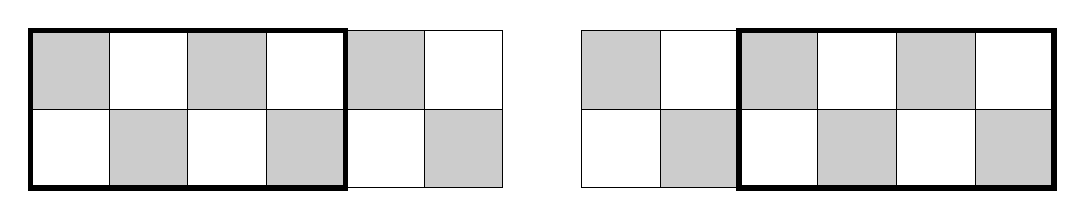
\begin{tikzpicture}

	\def \a {0}
	\def \b {0}
	\draw[fill=black!0!white] (\a,\b)--(\a+1,\b)--(\a+1,\b+1)--(\a,\b+1)--cycle;
	\def \a {1}
	\def \b {0}
	\draw[fill=black!20!white] (\a,\b)--(\a+1,\b)--(\a+1,\b+1)--(\a,\b+1)--cycle;
	\def \a {2}
	\def \b {0}
	\draw[fill=black!0!white] (\a,\b)--(\a+1,\b)--(\a+1,\b+1)--(\a,\b+1)--cycle;
	\def \a {3}
	\def \b {0}
	\draw[fill=black!20!white] (\a,\b)--(\a+1,\b)--(\a+1,\b+1)--(\a,\b+1)--cycle;
	\def \a {4}
	\def \b {0}
	\draw[fill=black!0!white] (\a,\b)--(\a+1,\b)--(\a+1,\b+1)--(\a,\b+1)--cycle;
	\def \a {5}
	\def \b {0}
	\draw[fill=black!20!white] (\a,\b)--(\a+1,\b)--(\a+1,\b+1)--(\a,\b+1)--cycle;
	\def \a {0}
	\def \b {1}
	\draw[fill=black!20!white] (\a,\b)--(\a+1,\b)--(\a+1,\b+1)--(\a,\b+1)--cycle;
	\def \a {1}
	\def \b {1}
	\draw[fill=black!0!white] (\a,\b)--(\a+1,\b)--(\a+1,\b+1)--(\a,\b+1)--cycle;
	\def \a {2}
	\def \b {1}
	\draw[fill=black!20!white] (\a,\b)--(\a+1,\b)--(\a+1,\b+1)--(\a,\b+1)--cycle;
	\def \a {3}
	\def \b {1}
	\draw[fill=black!0!white] (\a,\b)--(\a+1,\b)--(\a+1,\b+1)--(\a,\b+1)--cycle;
	\def \a {4}
	\def \b {1}
	\draw[fill=black!20!white] (\a,\b)--(\a+1,\b)--(\a+1,\b+1)--(\a,\b+1)--cycle;
	\def \a {5}
	\def \b {1}
	\draw[fill=black!0!white] (\a,\b)--(\a+1,\b)--(\a+1,\b+1)--(\a,\b+1)--cycle;
	
	\draw[line width=2] (0,0)--(4,0)--(4,2)--(0,2)--cycle;


\begin{scope}[xshift=7cm]

	\def \a {0}
	\def \b {0}
	\draw[fill=black!0!white] (\a,\b)--(\a+1,\b)--(\a+1,\b+1)--(\a,\b+1)--cycle;
	\def \a {1}
	\def \b {0}
	\draw[fill=black!20!white] (\a,\b)--(\a+1,\b)--(\a+1,\b+1)--(\a,\b+1)--cycle;
	\def \a {2}
	\def \b {0}
	\draw[fill=black!0!white] (\a,\b)--(\a+1,\b)--(\a+1,\b+1)--(\a,\b+1)--cycle;
	\def \a {3}
	\def \b {0}
	\draw[fill=black!20!white] (\a,\b)--(\a+1,\b)--(\a+1,\b+1)--(\a,\b+1)--cycle;
	\def \a {4}
	\def \b {0}
	\draw[fill=black!0!white] (\a,\b)--(\a+1,\b)--(\a+1,\b+1)--(\a,\b+1)--cycle;
	\def \a {5}
	\def \b {0}
	\draw[fill=black!20!white] (\a,\b)--(\a+1,\b)--(\a+1,\b+1)--(\a,\b+1)--cycle;
	\def \a {0}
	\def \b {1}
	\draw[fill=black!20!white] (\a,\b)--(\a+1,\b)--(\a+1,\b+1)--(\a,\b+1)--cycle;
	\def \a {1}
	\def \b {1}
	\draw[fill=black!0!white] (\a,\b)--(\a+1,\b)--(\a+1,\b+1)--(\a,\b+1)--cycle;
	\def \a {2}
	\def \b {1}
	\draw[fill=black!20!white] (\a,\b)--(\a+1,\b)--(\a+1,\b+1)--(\a,\b+1)--cycle;
	\def \a {3}
	\def \b {1}
	\draw[fill=black!0!white] (\a,\b)--(\a+1,\b)--(\a+1,\b+1)--(\a,\b+1)--cycle;
	\def \a {4}
	\def \b {1}
	\draw[fill=black!20!white] (\a,\b)--(\a+1,\b)--(\a+1,\b+1)--(\a,\b+1)--cycle;
	\def \a {5}
	\def \b {1}
	\draw[fill=black!0!white] (\a,\b)--(\a+1,\b)--(\a+1,\b+1)--(\a,\b+1)--cycle;
	
	\draw[line width=2] (2,0)--(6,0)--(6,2)--(2,2)--cycle;

\end{scope}

\end{tikzpicture} \\  \\
So again $Z(2 \times 4) = 5$ and $Z(2 \times 2) = 2$ and we should patch these together to obtain $Z (2 \times 6) = 13$.  Is that right? \\

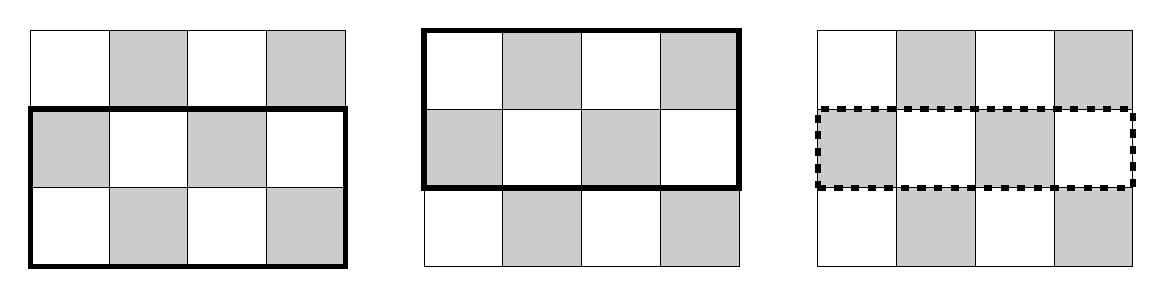
\begin{tikzpicture}

	\def \a {0}
	\def \b {0}
	\draw[fill=black!0!white] (\a,\b)--(\a+1,\b)--(\a+1,\b+1)--(\a,\b+1)--cycle;
	\def \a {1}
	\def \b {0}
	\draw[fill=black!20!white] (\a,\b)--(\a+1,\b)--(\a+1,\b+1)--(\a,\b+1)--cycle;
	\def \a {2}
	\def \b {0}
	\draw[fill=black!0!white] (\a,\b)--(\a+1,\b)--(\a+1,\b+1)--(\a,\b+1)--cycle;
	\def \a {3}
	\def \b {0}
	\draw[fill=black!20!white] (\a,\b)--(\a+1,\b)--(\a+1,\b+1)--(\a,\b+1)--cycle;
	\def \a {0}
	\def \b {1}
	\draw[fill=black!20!white] (\a,\b)--(\a+1,\b)--(\a+1,\b+1)--(\a,\b+1)--cycle;
	\def \a {1}
	\def \b {1}
	\draw[fill=black!0!white] (\a,\b)--(\a+1,\b)--(\a+1,\b+1)--(\a,\b+1)--cycle;
	\def \a {2}
	\def \b {1}
	\draw[fill=black!20!white] (\a,\b)--(\a+1,\b)--(\a+1,\b+1)--(\a,\b+1)--cycle;
	\def \a {3}
	\def \b {1}
	\draw[fill=black!0!white] (\a,\b)--(\a+1,\b)--(\a+1,\b+1)--(\a,\b+1)--cycle;
	\def \a {0}
	\def \b {2}
	\draw[fill=black!0!white] (\a,\b)--(\a+1,\b)--(\a+1,\b+1)--(\a,\b+1)--cycle;
	\def \a {1}
	\def \b {2}
	\draw[fill=black!20!white] (\a,\b)--(\a+1,\b)--(\a+1,\b+1)--(\a,\b+1)--cycle;
	\def \a {2}
	\def \b {2}
	\draw[fill=black!0!white] (\a,\b)--(\a+1,\b)--(\a+1,\b+1)--(\a,\b+1)--cycle;
	\def \a {3}
	\def \b {2}
	\draw[fill=black!20!white] (\a,\b)--(\a+1,\b)--(\a+1,\b+1)--(\a,\b+1)--cycle;
	
	\draw[line width=2] (0,0)--(4,0)--(4,2)--(0,2)--cycle;

\begin{scope}[xshift=5cm]

	\def \a {0}
	\def \b {0}
	\draw[fill=black!0!white] (\a,\b)--(\a+1,\b)--(\a+1,\b+1)--(\a,\b+1)--cycle;
	\def \a {1}
	\def \b {0}
	\draw[fill=black!20!white] (\a,\b)--(\a+1,\b)--(\a+1,\b+1)--(\a,\b+1)--cycle;
	\def \a {2}
	\def \b {0}
	\draw[fill=black!0!white] (\a,\b)--(\a+1,\b)--(\a+1,\b+1)--(\a,\b+1)--cycle;
	\def \a {3}
	\def \b {0}
	\draw[fill=black!20!white] (\a,\b)--(\a+1,\b)--(\a+1,\b+1)--(\a,\b+1)--cycle;
	\def \a {0}
	\def \b {1}
	\draw[fill=black!20!white] (\a,\b)--(\a+1,\b)--(\a+1,\b+1)--(\a,\b+1)--cycle;
	\def \a {1}
	\def \b {1}
	\draw[fill=black!0!white] (\a,\b)--(\a+1,\b)--(\a+1,\b+1)--(\a,\b+1)--cycle;
	\def \a {2}
	\def \b {1}
	\draw[fill=black!20!white] (\a,\b)--(\a+1,\b)--(\a+1,\b+1)--(\a,\b+1)--cycle;
	\def \a {3}
	\def \b {1}
	\draw[fill=black!0!white] (\a,\b)--(\a+1,\b)--(\a+1,\b+1)--(\a,\b+1)--cycle;
	\def \a {0}
	\def \b {2}
	\draw[fill=black!0!white] (\a,\b)--(\a+1,\b)--(\a+1,\b+1)--(\a,\b+1)--cycle;
	\def \a {1}
	\def \b {2}
	\draw[fill=black!20!white] (\a,\b)--(\a+1,\b)--(\a+1,\b+1)--(\a,\b+1)--cycle;
	\def \a {2}
	\def \b {2}
	\draw[fill=black!0!white] (\a,\b)--(\a+1,\b)--(\a+1,\b+1)--(\a,\b+1)--cycle;
	\def \a {3}
	\def \b {2}
	\draw[fill=black!20!white] (\a,\b)--(\a+1,\b)--(\a+1,\b+1)--(\a,\b+1)--cycle;
	
	\draw[line width=2] (0,1)--(4,1)--(4,3)--(0,3)--cycle;


\end{scope}

\begin{scope}[xshift=10cm]

	\def \a {0}
	\def \b {0}
	\draw[fill=black!0!white] (\a,\b)--(\a+1,\b)--(\a+1,\b+1)--(\a,\b+1)--cycle;
	\def \a {1}
	\def \b {0}
	\draw[fill=black!20!white] (\a,\b)--(\a+1,\b)--(\a+1,\b+1)--(\a,\b+1)--cycle;
	\def \a {2}
	\def \b {0}
	\draw[fill=black!0!white] (\a,\b)--(\a+1,\b)--(\a+1,\b+1)--(\a,\b+1)--cycle;
	\def \a {3}
	\def \b {0}
	\draw[fill=black!20!white] (\a,\b)--(\a+1,\b)--(\a+1,\b+1)--(\a,\b+1)--cycle;
	\def \a {0}
	\def \b {1}
	\draw[fill=black!20!white] (\a,\b)--(\a+1,\b)--(\a+1,\b+1)--(\a,\b+1)--cycle;
	\def \a {1}
	\def \b {1}
	\draw[fill=black!0!white] (\a,\b)--(\a+1,\b)--(\a+1,\b+1)--(\a,\b+1)--cycle;
	\def \a {2}
	\def \b {1}
	\draw[fill=black!20!white] (\a,\b)--(\a+1,\b)--(\a+1,\b+1)--(\a,\b+1)--cycle;
	\def \a {3}
	\def \b {1}
	\draw[fill=black!0!white] (\a,\b)--(\a+1,\b)--(\a+1,\b+1)--(\a,\b+1)--cycle;
	\def \a {0}
	\def \b {2}
	\draw[fill=black!0!white] (\a,\b)--(\a+1,\b)--(\a+1,\b+1)--(\a,\b+1)--cycle;
	\def \a {1}
	\def \b {2}
	\draw[fill=black!20!white] (\a,\b)--(\a+1,\b)--(\a+1,\b+1)--(\a,\b+1)--cycle;
	\def \a {2}
	\def \b {2}
	\draw[fill=black!0!white] (\a,\b)--(\a+1,\b)--(\a+1,\b+1)--(\a,\b+1)--cycle;
	\def \a {3}
	\def \b {2}
	\draw[fill=black!20!white] (\a,\b)--(\a+1,\b)--(\a+1,\b+1)--(\a,\b+1)--cycle;
	
	\draw[dashed, line width=2] (0,1)--(4,1)--(4,2)--(0,2)--cycle;


\end{scope}

\end{tikzpicture} \\ \\
The $3 \times n$ or $4 \times n$ cases deserve attention and could be pedagogical.  We will have more observables to think about soon.  And one should already be thinking about whether domino tilings are the only cases we can reasonably solve.  That answer might be yes \dots

\fontfamily{qag}\selectfont \fontsize{20}{25}\selectfont

\newpage Let's try to evaluate the $3 \times 4$ case.  The Kasteleyn matrix should be $6 \times 6$:

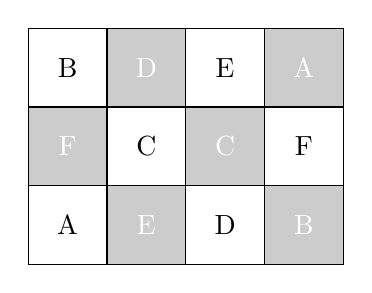
\begin{tikzpicture}

	\def \a {0}
	\def \b {0}
	\draw[fill=black!0!white] (\a,\b)--(\a+1,\b)--(\a+1,\b+1)--(\a,\b+1)--cycle;
	\def \a {1}
	\def \b {0}
	\draw[fill=black!20!white] (\a,\b)--(\a+1,\b)--(\a+1,\b+1)--(\a,\b+1)--cycle;
	\def \a {2}
	\def \b {0}
	\draw[fill=black!0!white] (\a,\b)--(\a+1,\b)--(\a+1,\b+1)--(\a,\b+1)--cycle;
	\def \a {3}
	\def \b {0}
	\draw[fill=black!20!white] (\a,\b)--(\a+1,\b)--(\a+1,\b+1)--(\a,\b+1)--cycle;
	\def \a {0}
	\def \b {1}
	\draw[fill=black!20!white] (\a,\b)--(\a+1,\b)--(\a+1,\b+1)--(\a,\b+1)--cycle;
	\def \a {1}
	\def \b {1}
	\draw[fill=black!0!white] (\a,\b)--(\a+1,\b)--(\a+1,\b+1)--(\a,\b+1)--cycle;
	\def \a {2}
	\def \b {1}
	\draw[fill=black!20!white] (\a,\b)--(\a+1,\b)--(\a+1,\b+1)--(\a,\b+1)--cycle;
	\def \a {3}
	\def \b {1}
	\draw[fill=black!0!white] (\a,\b)--(\a+1,\b)--(\a+1,\b+1)--(\a,\b+1)--cycle;
	\def \a {0}
	\def \b {2}
	\draw[fill=black!0!white] (\a,\b)--(\a+1,\b)--(\a+1,\b+1)--(\a,\b+1)--cycle;
	\def \a {1}
	\def \b {2}
	\draw[fill=black!20!white] (\a,\b)--(\a+1,\b)--(\a+1,\b+1)--(\a,\b+1)--cycle;
	\def \a {2}
	\def \b {2}
	\draw[fill=black!0!white] (\a,\b)--(\a+1,\b)--(\a+1,\b+1)--(\a,\b+1)--cycle;
	\def \a {3}
	\def \b {2}
	\draw[fill=black!20!white] (\a,\b)--(\a+1,\b)--(\a+1,\b+1)--(\a,\b+1)--cycle;
	
	\node at (0.5,0.5) {A};
	\node at (0.5,2.5) {B};
	\node at (1.5,1.5) {C};
	\node at (2.5,0.5) {D};
	\node at (2.5,2.5) {E};
	\node at (3.5,1.5) {F};

	\node at (3.5,2.5) {\color{white} A};
	\node at (3.5,0.5) {\color{white} B};
	\node at (2.5,1.5) {\color{white} C};
	\node at (1.5,2.5) {\color{white} D};
	\node at (1.5,0.5) {\color{white} E};
	\node at (0.5,1.5) {\color{white} F};

\end{tikzpicture} \\
I do \textbf{not} like matrix notation because the indices are themselves two-dimensionals A-,B-,C-,D-,E-,F- have information all around them.

$$ \det \left[ \begin{array}{cccccc} 
0 & 0 & 0 & 0 & 1 & 1 \\
0 & 0 & 0 & 1 & 0 & 1 \\
0 & 0 & 1 & 1 & 1 & 1 \\
0 & 1 & 1 & 0 & 1 & 0 \\
1 & 0 & 1 & 1 & 0 & 1 \\
1 & 1 & 1 & 0 & 0 & 0 

\end{array}\right] = 0$$
This is just like last time.  Determinant is zero\footnote{This could be that rectangle has trivial homology.  There is rel}.  Except I am not sure where to put the signs $+1$ and $-1$.  If I recall the orentation comes from picking one of the tilings.

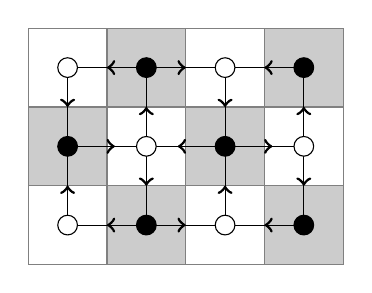
\begin{tikzpicture}

	\def \a {0}
	\def \b {0}
	\draw[black!50!white, fill=black!0!white] (\a,\b)--(\a+1,\b)--(\a+1,\b+1)--(\a,\b+1)--cycle;
	\def \a {1}
	\def \b {0}
	\draw[black!50!white,fill=black!20!white] (\a,\b)--(\a+1,\b)--(\a+1,\b+1)--(\a,\b+1)--cycle;
	\def \a {2}
	\def \b {0}
	\draw[black!50!white,fill=black!0!white] (\a,\b)--(\a+1,\b)--(\a+1,\b+1)--(\a,\b+1)--cycle;
	\def \a {3}
	\def \b {0}
	\draw[black!50!white,fill=black!20!white] (\a,\b)--(\a+1,\b)--(\a+1,\b+1)--(\a,\b+1)--cycle;
	\def \a {0}
	\def \b {1}
	\draw[black!50!white,fill=black!20!white] (\a,\b)--(\a+1,\b)--(\a+1,\b+1)--(\a,\b+1)--cycle;
	\def \a {1}
	\def \b {1}
	\draw[black!50!white,fill=black!0!white] (\a,\b)--(\a+1,\b)--(\a+1,\b+1)--(\a,\b+1)--cycle;
	\def \a {2}
	\def \b {1}
	\draw[black!50!white,fill=black!20!white] (\a,\b)--(\a+1,\b)--(\a+1,\b+1)--(\a,\b+1)--cycle;
	\def \a {3}
	\def \b {1}
	\draw[black!50!white,fill=black!0!white] (\a,\b)--(\a+1,\b)--(\a+1,\b+1)--(\a,\b+1)--cycle;
	\def \a {0}
	\def \b {2}
	\draw[black!50!white,fill=black!0!white] (\a,\b)--(\a+1,\b)--(\a+1,\b+1)--(\a,\b+1)--cycle;
	\def \a {1}
	\def \b {2}
	\draw[black!50!white,fill=black!20!white] (\a,\b)--(\a+1,\b)--(\a+1,\b+1)--(\a,\b+1)--cycle;
	\def \a {2}
	\def \b {2}
	\draw[black!50!white,fill=black!0!white] (\a,\b)--(\a+1,\b)--(\a+1,\b+1)--(\a,\b+1)--cycle;
	\def \a {3}
	\def \b {2}
	\draw[black!50!white,fill=black!20!white] (\a,\b)--(\a+1,\b)--(\a+1,\b+1)--(\a,\b+1)--cycle;
	
	
	\draw[decoration={markings, mark=at position 0.5 with {\arrow[scale=1,  line width=1]{>}}},
        postaction={decorate}] (1.5,0.5)--(0.5,0.5);
	\draw[decoration={markings, mark=at position 0.5 with {\arrow[scale=1,  line width=1]{>}}},
        postaction={decorate}] (3.5,0.5)--(2.5,0.5);
	\draw[decoration={markings, mark=at position 0.6 with {\arrow[scale=1,  line width=1]{>}}},
        postaction={decorate}] (0.5,1.5)--(1.5,1.5);
	\draw[decoration={markings, mark=at position 0.6 with {\arrow[scale=1,  line width=1]{>}}},
        postaction={decorate}] (2.5,1.5)--(3.5,1.5);
	\draw[decoration={markings, mark=at position 0.5 with {\arrow[scale=1,  line width=1]{>}}},
        postaction={decorate}] (1.5,2.5)--(0.5,2.5);
	\draw[decoration={markings, mark=at position 0.5 with {\arrow[scale=1,  line width=1]{>}}},
        postaction={decorate}] (3.5,2.5)--(2.5,2.5);
	\draw[decoration={markings, mark=at position 0.5 with {\arrow[scale=1,  line width=1]{>}}},
        postaction={decorate}] (1.5,0.5)--(2.5,0.5);
	\draw[decoration={markings, mark=at position 0.6 with {\arrow[scale=1,  line width=1]{>}}},
        postaction={decorate}] (2.5,1.5)--(1.5,1.5);        
	\draw[decoration={markings, mark=at position 0.5 with {\arrow[scale=1,  line width=1]{>}}},
        postaction={decorate}] (1.5,2.5)--(2.5,2.5);         
        
        
        
	\draw[decoration={markings, mark=at position 0.5 with {\arrow[scale=1,  line width=1]{>}}},
        postaction={decorate}] (0.5,0.5)--(0.5,1.5);
	\draw[decoration={markings, mark=at position 0.5 with {\arrow[scale=1,  line width=1]{>}}},
        postaction={decorate}] (0.5,2.5)--(0.5,1.5);
	\draw[decoration={markings, mark=at position 0.5 with {\arrow[scale=1,  line width=1]{>}}},
        postaction={decorate}] (1.5,1.5)--(1.5,0.5);
	\draw[decoration={markings, mark=at position 0.5 with {\arrow[scale=1,  line width=1]{>}}},
        postaction={decorate}] (1.5,1.5)--(1.5,2.5);
	\draw[decoration={markings, mark=at position 0.5 with {\arrow[scale=1,  line width=1]{>}}},
        postaction={decorate}] (2.5,0.5)--(2.5,1.5);
	\draw[decoration={markings, mark=at position 0.5 with {\arrow[scale=1,  line width=1]{>}}},
        postaction={decorate}] (2.5,2.5)--(2.5,1.5);
	\draw[decoration={markings, mark=at position 0.5 with {\arrow[scale=1,  line width=1]{>}}},
        postaction={decorate}] (3.5,1.5)--(3.5,0.5);
	\draw[decoration={markings, mark=at position 0.5 with {\arrow[scale=1,  line width=1]{>}}},
        postaction={decorate}] (3.5,1.5)--(3.5,2.5);
	
	\draw[fill=white] (0.5,0.5) circle (0.125);
	\draw[fill=white] (2.5,0.5) circle (0.125);
	\draw[fill=white] (1.5,1.5) circle (0.125);
	\draw[fill=white] (0.5,2.5) circle (0.125);
	\draw[fill=white] (2.5,2.5) circle (0.125);
	\draw[fill=white] (3.5,1.5) circle (0.125);
	
	\draw[fill=black] (1.5,0.5) circle (0.125);
	\draw[fill=black] (3.5,0.5) circle (0.125);
	\draw[fill=black] (0.5,1.5) circle (0.125);
	\draw[fill=black] (2.5,1.5) circle (0.125);
	\draw[fill=black] (1.5,2.5) circle (0.125);
	\draw[fill=black] (3.5,2.5) circle (0.125);
	
\end{tikzpicture} \\
It was pretty exhausting to type this.  Because there is a lot of structure that goes into drawing a very simple shape.

\newpage

$$
\det \left[
\begin{array}{rrrrrr} 
0 & 0 & 0 & 0 & 1 & -1 \\
0 & 0 & 0 & 1 & 0 & -1 \\
0 & 0 & 1 & -1 & -1 & 1 \\
0 & 1 & -1 & 0 & 1 & 0 \\
1 & 0 & -1 & 1 & 0 & 1 \\
-1 & -1 & 1 & 0 & 0 & 0  \end{array}
\right] = 2 \neq 11 $$
Time to read a bit more on Kasteleyn orientations.  OK It's done with a spanning tree.

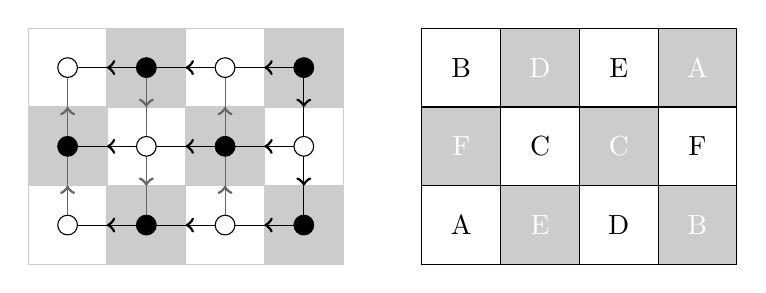
\begin{tikzpicture}

	\def \a {0}
	\def \b {0}
	\draw[black!20!white, fill=black!0!white] (\a,\b)--(\a+1,\b)--(\a+1,\b+1)--(\a,\b+1)--cycle;
	\def \a {1}
	\def \b {0}
	\draw[black!20!white,fill=black!20!white] (\a,\b)--(\a+1,\b)--(\a+1,\b+1)--(\a,\b+1)--cycle;
	\def \a {2}
	\def \b {0}
	\draw[black!20!white,fill=black!0!white] (\a,\b)--(\a+1,\b)--(\a+1,\b+1)--(\a,\b+1)--cycle;
	\def \a {3}
	\def \b {0}
	\draw[black!20!white,fill=black!20!white] (\a,\b)--(\a+1,\b)--(\a+1,\b+1)--(\a,\b+1)--cycle;
	\def \a {0}
	\def \b {1}
	\draw[black!20!white,fill=black!20!white] (\a,\b)--(\a+1,\b)--(\a+1,\b+1)--(\a,\b+1)--cycle;
	\def \a {1}
	\def \b {1}
	\draw[black!20!white,fill=black!0!white] (\a,\b)--(\a+1,\b)--(\a+1,\b+1)--(\a,\b+1)--cycle;
	\def \a {2}
	\def \b {1}
	\draw[black!20!white,fill=black!20!white] (\a,\b)--(\a+1,\b)--(\a+1,\b+1)--(\a,\b+1)--cycle;
	\def \a {3}
	\def \b {1}
	\draw[black!20!white,fill=black!0!white] (\a,\b)--(\a+1,\b)--(\a+1,\b+1)--(\a,\b+1)--cycle;
	\def \a {0}
	\def \b {2}
	\draw[black!20!white,fill=black!0!white] (\a,\b)--(\a+1,\b)--(\a+1,\b+1)--(\a,\b+1)--cycle;
	\def \a {1}
	\def \b {2}
	\draw[black!20!white,fill=black!20!white] (\a,\b)--(\a+1,\b)--(\a+1,\b+1)--(\a,\b+1)--cycle;
	\def \a {2}
	\def \b {2}
	\draw[black!20!white,fill=black!0!white] (\a,\b)--(\a+1,\b)--(\a+1,\b+1)--(\a,\b+1)--cycle;
	\def \a {3}
	\def \b {2}
	\draw[black!20!white,fill=black!20!white] (\a,\b)--(\a+1,\b)--(\a+1,\b+1)--(\a,\b+1)--cycle;
	
	
	\draw[decoration={markings, mark=at position 0.5 with {\arrow[scale=1,  line width=1]{>}}},
        postaction={decorate}] (1.5,0.5)--(0.5,0.5);        
	\draw[decoration={markings, mark=at position 0.5 with {\arrow[scale=1,  line width=1]{>}}},
        postaction={decorate}] (2.5,0.5)--(1.5,0.5);  
	\draw[decoration={markings, mark=at position 0.5 with {\arrow[scale=1,  line width=1]{>}}},
        postaction={decorate}] (3.5,0.5)--(2.5,0.5);  
	\draw[decoration={markings, mark=at position 0.5 with {\arrow[scale=1,  line width=1]{>}}},
        postaction={decorate}] (1.5,1.5)--(0.5,1.5);        
	\draw[decoration={markings, mark=at position 0.5 with {\arrow[scale=1,  line width=1]{>}}},
        postaction={decorate}] (2.5,1.5)--(1.5,1.5);  
	\draw[decoration={markings, mark=at position 0.5 with {\arrow[scale=1,  line width=1]{>}}},
        postaction={decorate}] (3.5,1.5)--(2.5,1.5); 
	\draw[decoration={markings, mark=at position 0.5 with {\arrow[scale=1,  line width=1]{>}}},
        postaction={decorate}] (1.5,2.5)--(0.5,2.5);        
	\draw[decoration={markings, mark=at position 0.5 with {\arrow[scale=1,  line width=1]{>}}},
        postaction={decorate}] (2.5,2.5)--(1.5,2.5);  
	\draw[decoration={markings, mark=at position 0.5 with {\arrow[scale=1,  line width=1]{>}}},
        postaction={decorate}] (3.5,2.5)--(2.5,2.5); 
	\draw[decoration={markings, mark=at position 0.5 with {\arrow[scale=1,  line width=1]{>}}},
        postaction={decorate}] (3.5,2.5)--(3.5,1.5);        
	\draw[decoration={markings, mark=at position 0.5 with {\arrow[scale=1,  line width=1]{>}}},
        postaction={decorate}] (3.5,1.5)--(3.5,0.5);          

	\draw[black!60!white,decoration={markings, mark=at position 0.5 with {\arrow[scale=1,  line width=1]{>}}},
        postaction={decorate}] (2.5,0.5)--(2.5,1.5);         
	\draw[black!60!white,decoration={markings, mark=at position 0.5 with {\arrow[scale=1,  line width=1]{>}}},
        postaction={decorate}] (1.5,1.5)--(1.5,0.5); 
	\draw[black!60!white,decoration={markings, mark=at position 0.5 with {\arrow[scale=1,  line width=1]{>}}},
        postaction={decorate}] (0.5,0.5)--(0.5,1.5); 
	\draw[black!60!white,decoration={markings, mark=at position 0.5 with {\arrow[scale=1,  line width=1]{>}}},
        postaction={decorate}] (2.5,1.5)--(2.5,2.5);         
	\draw[black!60!white,decoration={markings, mark=at position 0.5 with {\arrow[scale=1,  line width=1]{>}}},
        postaction={decorate}] (1.5,2.5)--(1.5,1.5); 
	\draw[black!60!white,decoration={markings, mark=at position 0.5 with {\arrow[scale=1,  line width=1]{>}}},
        postaction={decorate}] (0.5,1.5)--(0.5,2.5); 
	
	\draw[fill=white] (0.5,0.5) circle (0.125);
	\draw[fill=white] (2.5,0.5) circle (0.125);
	\draw[fill=white] (1.5,1.5) circle (0.125);
	\draw[fill=white] (0.5,2.5) circle (0.125);
	\draw[fill=white] (2.5,2.5) circle (0.125);
	\draw[fill=white] (3.5,1.5) circle (0.125);
	
	\draw[fill=black] (1.5,0.5) circle (0.125);
	\draw[fill=black] (3.5,0.5) circle (0.125);
	\draw[fill=black] (0.5,1.5) circle (0.125);
	\draw[fill=black] (2.5,1.5) circle (0.125);
	\draw[fill=black] (1.5,2.5) circle (0.125);
	\draw[fill=black] (3.5,2.5) circle (0.125);
	
	
\begin{scope}[xshift=5cm]


	\def \a {0}
	\def \b {0}

	\draw[fill=black!0!white] (\a,\b)--(\a+1,\b)--(\a+1,\b+1)--(\a,\b+1)--cycle;
	\def \a {1}
	\def \b {0}
	\draw[fill=black!20!white] (\a,\b)--(\a+1,\b)--(\a+1,\b+1)--(\a,\b+1)--cycle;
	\def \a {2}
	\def \b {0}
	\draw[fill=black!0!white] (\a,\b)--(\a+1,\b)--(\a+1,\b+1)--(\a,\b+1)--cycle;
	\def \a {3}
	\def \b {0}
	\draw[fill=black!20!white] (\a,\b)--(\a+1,\b)--(\a+1,\b+1)--(\a,\b+1)--cycle;
	\def \a {0}
	\def \b {1}
	\draw[fill=black!20!white] (\a,\b)--(\a+1,\b)--(\a+1,\b+1)--(\a,\b+1)--cycle;
	\def \a {1}
	\def \b {1}
	\draw[fill=black!0!white] (\a,\b)--(\a+1,\b)--(\a+1,\b+1)--(\a,\b+1)--cycle;
	\def \a {2}
	\def \b {1}
	\draw[fill=black!20!white] (\a,\b)--(\a+1,\b)--(\a+1,\b+1)--(\a,\b+1)--cycle;
	\def \a {3}
	\def \b {1}
	\draw[fill=black!0!white] (\a,\b)--(\a+1,\b)--(\a+1,\b+1)--(\a,\b+1)--cycle;
	\def \a {0}
	\def \b {2}
	\draw[fill=black!0!white] (\a,\b)--(\a+1,\b)--(\a+1,\b+1)--(\a,\b+1)--cycle;
	\def \a {1}
	\def \b {2}
	\draw[fill=black!20!white] (\a,\b)--(\a+1,\b)--(\a+1,\b+1)--(\a,\b+1)--cycle;
	\def \a {2}
	\def \b {2}
	\draw[fill=black!0!white] (\a,\b)--(\a+1,\b)--(\a+1,\b+1)--(\a,\b+1)--cycle;
	\def \a {3}
	\def \b {2}
	\draw[fill=black!20!white] (\a,\b)--(\a+1,\b)--(\a+1,\b+1)--(\a,\b+1)--cycle;
	
	\node at (0.5,0.5) {A};
	\node at (0.5,2.5) {B};
	\node at (1.5,1.5) {C};
	\node at (2.5,0.5) {D};
	\node at (2.5,2.5) {E};
	\node at (3.5,1.5) {F};

	\node at (3.5,2.5) {\color{white} A};
	\node at (3.5,0.5) {\color{white} B};
	\node at (2.5,1.5) {\color{white} C};
	\node at (1.5,2.5) {\color{white} D};
	\node at (1.5,0.5) {\color{white} E};
	\node at (0.5,1.5) {\color{white} F};
\end{scope}
	
	
\end{tikzpicture} \\
As you move around the square, there should be either
\begin{itemize}
\item 3 $\leftarrow$, 1 $\rightarrow$
\item 1 $\leftarrow$, 3 $\rightarrow$
\end{itemize}
and in some cases these are called ``IRF" models (interaction around face).  I also have a round face.
$$ \det \left[
\begin{array}{rrrrrrr}
0 & 0& 0& 0& +1& +1\\
0 & 0 & 0 & +1 & 0 & -1 \\
0 & 0 & +1 & -1 & +1 & -1 \\
0 & +1 & +1 & 0 & -1 & 0  \\
+1 & 0 & -1 & -1 & 0 & 0 \\
-1 & +1 & -1 & 0 & 0 & 0
\end{array}
 \right] = 11 $$
\hfill $\square$

\newpage

\fontfamily{qag}\selectfont \fontsize{12}{10}\selectfont

\noindent Can the physics literature offer more interesting tiling models?  Lots of overloaded terms here:
\begin{itemize}
\item domino tiling
\item dimer model
\end{itemize}
The dimer model is more general (since any planar graph has a dual tiling model), but maybe not all tiling problems come from a dimer model (the shapes can be more varied). \\ \\
The physics papers I raise more distinctions.  There's distinction between:
\begin{itemize}
\item high-energy physics (such as Chern Simons Theory)
\item condensed matter physics (such as TQFT, symmetry protected topological phases, ising models or free fermions)
\end{itemize}
This is consistent with using Gauge Theory to describe the theory of everything.  Here we are using Gauge Theory to describe the dominoes.  In th case we find the ising model there is one more distinction:
\begin{itemize}
\item ising statistical model (state-sum model)
\item ising conformal field theory (continuum limit)
\end{itemize}
Hopefully that is enough.  I am not sure I care which Chern-Simons Theories have tiling models as low-energy limits, as long as I know that Kasteleyn determinants are discrete Diract operators.
$$ \#\{\text{ tilings }\} = \det K  \approx \det \slashed{D} $$
I think the number of tilings is the factor of the Dirac determinant which gets thrown away (``renormalized"). \\ \\
Here is a really basic one if we define $\Delta f = \frac{1}{\Delta x}[f(x+\Delta x) - f(x)]$ then we discrete approximation:
$$ \frac{d}{dx} \approx \frac{1}{\Delta x} \left[  
\begin{array}{rrrr} 
1 & -1 & 0 &  \\
0 & 1 & -1 & 0 \\ 
 & 0 & \ddots & -1  \\
 &  & 0 & 1 
\end{array}\right] $$
In the same way, all these circulant matrices are discretizations of differential operators (maybe Dirac operators, for fermions) or whatever complicated thing that solves Chern-Simons Theory.

\fontfamily{qag}\selectfont \fontsize{12}{10}\selectfont

\begin{thebibliography}{}

\item Davide Gaiotto, Anton Kapustin \textbf{Spin TQFTs and fermionic phases of matter} \texttt{arXiv:1505.05856}

\item Nathan Seiberg, Edward Witten \textbf{Gapped Boundary Phases of Topological Insulators via Weak Coupling}   \texttt{arXiv:1602.04251}

\item Davide Gaiotto, Anton Kapustin, Zohar Komargodski, Nathan Seiberg \textbf{Theta, Time Reversal, and Temperature} \texttt{arXiv:1703.00501}

\item Edward Witten \textbf{Fermion Path Integrals And Topological Phases} \texttt{arXiv:1508.04715}

\item Nathan Seiberg, Edward Witten \textbf{Gapped Boundary Phases of Topological Insulators via Weak Coupling} \texttt{arXiv:1602.04251}

\item Werner Krauth \textbf{Statistical Mechanics: Algorithms and Computations} (Oxford Master Series in Physics), OUP, 2006.

\end{thebibliography} 

\vfill

\noindent The most amazing typo ever: \\

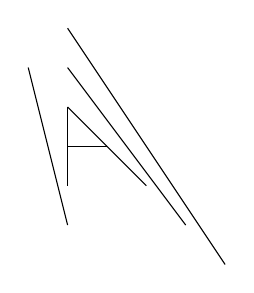
\begin{tikzpicture} [scale=0.5]

\foreach \a in {0,...,5}{
    \draw (\a,5-\a)--(1, \a + 1);
}

\end{tikzpicture}

\begin{verbatim}
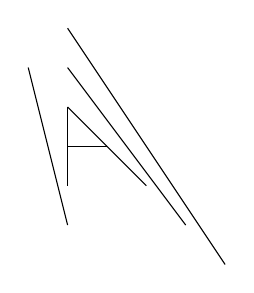
\begin{tikzpicture} [scale=0.5]

\foreach \a in {0,...,5}{

    \draw (\a, 5-\a)--(1, \a + 1);

}

\end{tikzpicture}
\end{verbatim}


\end{document}